% ASTRA RASTI Paper V1.17 — 2026-04-23
% Changes: Architecture diagram (P0), Table 1 extended to TC6+TC7 (P0),
%          TC7 figures to figure* (P1), bias char. fig added (P1),
%          test06_genuine_discovery.png added (P1), Kumar+2025 W3 B-field (TC7 PI),
%          LtU-ILI/FluxMC/StarWhisper added to Related Work (P1).
%          '15 test cases' overclaim fixed. Arch. fig cross-ref added.
% P0 fixes: bib errors (jin2025 DOI/author/title, desmond2026 coauthor/algorithm/DOI),
%            itemize→description, table captions above tabular, table 2 label added,
%            running head shortened, "lower bounds"→"upper bounds", "BIC-penalized"→"HME-estimated",
%            "FCI causal discovery"→"PC-algorithm causal discovery", FCI→FCIT for Desmond2026,
%            "six"→"seven" test cases, section numbers fixed, TC7 added to intro list.
% P1 fixes: Moss 2025 AI Cosmologist cited, \citealt→\citet, \cite→\citep (GitHub),
%            kass1995 nested-sampling citation → skilling2004, geometric factor removed,
%            TC6 outlier tally grammar fixed, mucesh2024 title corrected.
\documentclass[usenatbib]{rasti}

\usepackage{graphicx}
\usepackage{amsmath}
\usepackage{amssymb}
\usepackage{url}

\title[ASTRA: Autonomous Astrophysical Discovery]{ASTRA: Autonomous Scientific Discovery in Astrophysics}
\author[White]{
Glenn J.~White$^{1,2}$\thanks{E-mail: glenn.white@open.ac.uk}\\
$^{1}$Department of Physics and Astronomy, The Open University, Milton Keynes MK7~6AA, UK\\
$^{2}$RAL Space, STFC Rutherford Appleton Laboratory, Chilton, Didcot, Oxfordshire, OX11~0QX, UK
}

\begin{document}

\pubyear{2026}

\maketitle

\label{firstpage}

\begin{keywords}
methods: data analysis --- methods: statistical --- ISM: structure --- galaxies: general --- software: public release
\end{keywords}

\begin{abstract}
We present ASTRA (Autonomous System for Scientific Discovery in Astrophysics), an integrated framework combining numerical data analysis, causal reasoning, and physical validation. ASTRA integrates: dimensional analysis; structural causal models; Bayesian evidence computation; and multi-wavelength data fusion within a unified framework.

We demonstrate capabilities through seven test cases. The first five use real observational data to validate ASTRA's ability to recover known astrophysical results, including: Herschel filament scaling relations with dimensional analysis; Chandra Deep Field South multi-wavelength cross-matching with Bayesian uncertainty propagation; SDSS galaxy property correlations; Gaia stellar causal inference; and Bayesian model selection for virial scaling relations.

The sixth test case demonstrates discovery-mode operation on realistic galaxy survey data (3,000 galaxies based on SDSS scaling relations). ASTRA recovers the star-forming main sequence and mass-metallicity relation, then applies multi-dimensional outlier detection to identify starbursts, post-starbursts, and transitioning galaxies.

The seventh test case demonstrates autonomous HPC simulation campaign management: ASTRA co-ordinated 600+ Athena++ MHD simulations on a remote 224-vCPU server to validate the magnetic Jeans fragmentation criterion for ISM filaments, confirming the predicted stability threshold $\beta_\mathrm{crit} = 2/3$ and calibrating the fragmentation wavelength to $(1.11 \pm 0.12)\,\lambda_{J,m}(\theta,\beta)$ across 18 field-geometry configurations.

Code and documentation: \url{https://github.com/web3guru888/ASTRA} \citep{astra_github}.
\end{abstract}

\section{Introduction}

Modern astronomical surveys generate petabytes of data requiring automated analysis. Multiple computational approaches are available to astronomers, each with distinct strengths and limitations.

\textbf{Traditional Machine Learning and Statistical Methods}: Well-established tools including scikit-learn, emcee, and nested sampling codes (MultiNest, dynesty) can process numerical data, detect patterns, perform statistical inference, and compute Bayesian evidence. These methods are widely used in astronomy with demonstrated success.

\textbf{Large Language Models with Code Execution}: Current frontier models (GPT-4 with Code Interpreter, Claude with code execution) can process numerical data, execute Python code, and perform statistical analysis. These systems provide conversational interfaces to computational tools but require explicit programming and do not natively integrate physical validation or causal interpretation.

\textbf{The Integration Challenge}: While individual tools exist for specific tasks, astronomers typically must manually combine separate pipelines for data processing, statistical analysis, causal inference, and physical validation. This manual integration creates opportunities for inconsistent treatment of uncertainties, missed physical constraints, and difficulty reproducing multi-step analyses.

ASTRA addresses this challenge by providing an integrated framework that combines:
\begin{description}
\item[] Numerical data processing and statistical analysis
\item[] Causal reasoning with structural causal models
\item[] Physical validation through dimensional analysis and conservation laws
\item[] Multi-wavelength data fusion with uncertainty propagation
\item[] Hypothesis generation from pattern recognition
\item[] Bayesian model selection with evidence computation
\end{description}

This integrated approach provides a unified framework where physical validation, causal reasoning, and uncertainty quantification are applied consistently throughout multi-step analyses. While individual components use established algorithms (PC algorithm for causal discovery, marginal likelihood estimation for Bayesian evidence, dimensional analysis for physical validation), their integration within a single framework enables analyses that would otherwise require manual combination of multiple separate tools.

In this paper, we focus on seven examples demonstrating how this integrated approach can be applied to astrophysical inference problems:
\begin{enumerate}
\item \textbf{Scaling Relations Analysis} (Section~3): Dimensional analysis and physical validation of filament scaling relations
\item \textbf{Multi-Wavelength Data Fusion} (Section~4): Probabilistic cross-matching with Bayesian uncertainty propagation
\item \textbf{Pattern Recognition} (Section~5): Identification of established galaxy property relationships
\item \textbf{Causal Inference} (Section~6): Structural causal model discovery in stellar data
\item \textbf{Bayesian Model Selection} (Section~7): Evidence-based model comparison with prior specification
\item \textbf{Discovery-Mode Analysis} (Section~8): Galaxy scaling relations and outlier detection on realistic survey data
\item \textbf{Autonomous HPC Campaign} (Section~9): Autonomous MHD simulation campaign management for ISM filament fragmentation
\end{enumerate}

\textbf{Tests 1--5 use real observational data}, validating ASTRA's ability to correctly recover known astrophysical results. Test 6 uses realistic galaxy survey data based on SDSS scaling relations to demonstrate both validation (recovering known relations) and discovery (identifying outliers).

Section~10 discusses why these results demonstrate ASTRA's unique capabilities, clarifies ASTRA's role as a tool to assist rather than replace astronomers, and Section~11 concludes.

\subsection{Scope and Limitations}

\textbf{What ASTRA Demonstrates}: The seven test cases in this paper show ASTRA can: discover physical laws from data with theoretical validation; fuse multi-wavelength observations with proper uncertainty handling; identify established astrophysical relationships through pattern recognition; distinguish causation from correlation; perform rigorous Bayesian model comparison; and operate in discovery mode on realistic survey data to recover known relations while identifying unusual objects for follow-up.

\textbf{What ASTRA Does Not Claim}: ASTRA is not presented as achieving artificial general intelligence (AGI) or AGI-like performance. The system operates within defined astrophysical domains using established algorithms (PC-algorithm causal discovery, Bayesian inference, dimensional analysis) combined through an integrated architecture. Results are validated against known physical theory and observational constraints. The system does not claim general reasoning beyond its training domains or autonomous operation without human oversight. The architecture is designed to support natural language queries that trigger autonomous task completion, though this capability is not demonstrated in the present test cases.

\textbf{ASTRA's Role in Scientific Discovery}: We should not expect to give ASTRA one of the big contemporary problems like ``What is the nature of Dark Matter and Dark Energy,'' or ``How does gravity connect to quantum physics,'' or ``What sets the stellar initial mass function (IMF),'' and expect to get definitive answers that may be the equivalent of a computational Eureka moment. But ASTRA's discovery architecture, used alongside and by an experienced astronomer, has capabilities in discovery and inference that go beyond those of straightforward AI (large language models) and/or machine learning. ASTRA's role in science is to work alongside the experienced astronomer to analyze data and facilitate genuine discovery. ASTRA is therefore a tool to assist the astronomer, rather than a replacement for domain expertise.

\textbf{Validation Scope}: Tests 1--5 use real observational data to validate ASTRA's ability to correctly recover known astrophysical results. Test 6 uses realistic galaxy survey data based on published SDSS scaling relations to demonstrate both validation (recovering known relations) and discovery (identifying outliers). The data is generated using empirical relations from Kauffmann et al. (2003), Tremonti et al. (2004), and Brinchmann et al. (2004). The capabilities demonstrated are shown within specific astrophysical domains using particular datasets. Generalization to other domains or datasets requires further validation.

\section{Methods: ASTRA System Architecture}

\subsection{Overview}

ASTRA implements a modular architecture designed for astrophysical data analysis and inference. The system integrates multiple specialized components through a coordinated framework, enabling complex multi-step analyses that combine data processing, physical reasoning, causal inference, and statistical validation.

\subsection{Core Architectural Components}

\textbf{1. Data Processing Pipeline}: ASTRA accepts heterogeneous astronomical data formats including catalogs (CSV, FITS), time-series data, images, and spectral data. The pipeline performs ingestion, validation, cleaning, and normalization while preserving measurement uncertainties and metadata.

\textbf{2. Physics Engine}: A unified physics engine implements fundamental physical laws and constraints including conservation laws (mass, energy, momentum), dimensional analysis using Buckingham $\pi$ theorem, equation solving and numerical simulation, and units consistency checking throughout calculations. This enables ASTRA to validate discoveries against first principles rather than treating correlations as sufficient explanations.

\textbf{3. Causal Reasoning Module}: Implements causal discovery and inference using the PC algorithm \cite{spirtes2000} for discovering causal structures from observational data, conditional independence testing for continuous variables (Fisher's Z-test), V-structure detection for identifying colliders, do-calculus for predicting effects of interventions, and domain-specific adaptations for astrophysical contexts. This module enables ASTRA to distinguish causal relationships from correlations, addressing a fundamental limitation of both traditional ML and LLM approaches.

\textbf{4. Bayesian Inference Engine}: Implements rigorous model comparison and uncertainty quantification through evidence computation via marginal likelihood estimation, Bayes factors for model comparison \cite{kass1995}, automatic complexity penalty (Occam's razor), posterior predictive checking, and Monte Carlo methods for uncertainty propagation.

\textbf{5. Domain Knowledge Systems}: Organized astrophysical knowledge through MORK ontology encoding taxonomic and causal relationships, knowledge graphs for semantic relationships, vector-based semantic memory for concept retrieval, and 75 specialized domain modules (ISM, star formation, exoplanets, etc.).

\textbf{6. Multi-Module Orchestration}: Coordinates different analytical perspectives through specialized processing modules for different analysis types, meta-cognitive layer for context-appropriate module selection, result synthesis and conflict resolution, and quality control and validation checks.

\subsection{Unique Capabilities}

ASTRA integrates sixteen distinct analytical capabilities that work together to enable comprehensive scientific analysis:

\textbf{Causal and Statistical Analysis}: (1) \textit{Bias Detection}---Identifies and quantifies observational biases like Malmquist bias from survey geometry and selection effects. (2) \textit{Scaling Relations Discovery}---Discovers physical laws from data through dimensional analysis and functional form detection. (3) \textit{Causal Inference}---Discovers causal structures using the PC algorithm and distinguishes physical laws from selection biases. (4) \textit{Model Selection}---Compares competing theories using Bayesian evidence computation with proper complexity penalties.

\textbf{Data Integration and Analysis}: (5) \textit{Multi-Wavelength Fusion}---Cross-matches sources across wavelengths with proper astrometric uncertainty propagation. (6) \textit{Uncertainty Quantification}---Propagates measurement errors through first-order and Monte Carlo methods, separating systematic and statistical components. (7) \textit{Temporal Reasoning}---Detects periodic signals, performs phase folding, and forecasts time-series behavior. (8) \textit{Instrument-Aware Analysis}---Evaluates observational requirements and compatibility across multiple astronomical facilities.

\textbf{Knowledge Generation}: (9) \textit{Hypothesis Generation}---Identifies patterns, detects anomalies, and generates novel testable hypotheses with specific observational requirements. (10) \textit{Analogical Reasoning}---Discovers structural mappings between different astrophysical systems based on shared physics. (11) \textit{Counterfactual Analysis}---Simulates physically-grounded scenarios to predict effects of interventions or observational changes. (12) \textit{Physical Model Discovery}---Automatically identifies functional forms and validates against theoretical predictions.

\textbf{Meta-Cognitive Capabilities}: (13) \textit{Meta-Cognitive Evaluation}---Provides quantitative assessments of data sufficiency, resolution limits, and observational constraints. (14) \textit{Anomaly Detection}---Identifies unusual objects using ensemble methods combining multiple detection approaches. (15) \textit{Ensemble Prediction}---Combines multiple models using Bayesian Model Averaging for robust predictions with uncertainty quantification. (16) \textit{Physical Validation}---Checks all results against dimensional consistency, conservation laws, and established physical principles.

These capabilities are not independent modules but integrated components that work together. For example, discovering a scaling relation (capability~2) involves dimensional analysis (capability~12), physical validation (capability~16), and uncertainty quantification (capability~6). Similarly, multi-wavelength fusion (capability~5) requires coordinate calculations, astrometric error propagation, and physical classification criteria.

\textbf{Capability Demonstrations in This Paper}: Table~\ref{tab:capabilities} summarizes which of the 16 capabilities are demonstrated in each of the seven test cases. Capabilities not demonstrated in TCs~1--7 (temporal reasoning, instrument-aware analysis, analogical reasoning, counterfactual analysis, ensemble prediction) are available in ASTRA and demonstrated in extended test cases in the GitHub repository. TC7 additionally demonstrates a seventeenth capability (HPC simulation management) not listed in the 16-capability inventory.

\begin{table*}
\caption{Capabilities demonstrated in each test case. X~=~explicitly demonstrated; --~=~not demonstrated or not applicable. Temporal reasoning, instrument-aware analysis, analogical reasoning, counterfactual analysis, and ensemble prediction are available in ASTRA but demonstrated only in extended test cases on GitHub. TC7 additionally demonstrates HPC Simulation Management (row~17), a qualitatively distinct capability.}
\label{tab:capabilities}
\centering
\begin{tabular}{lccccccl}
\hline
Capability & TC1 & TC2 & TC3 & TC4 & TC5 & TC6 & TC7 \\
& (Scaling) & (Multi-$\lambda$) & (Pattern) & (Causal) & (Bayesian) & (Discovery) & (HPC MHD) \\
\hline
Bias Detection              & -- & X  & -- & X  & -- & -- & X  \\
Scaling Relations           & X  & -- & X  & -- & X  & X  & X  \\
Causal Inference            & -- & -- & -- & X  & -- & -- & -- \\
Model Selection             & -- & -- & -- & -- & X  & -- & -- \\
Multi-Wavelength Fusion     & -- & X  & -- & -- & -- & -- & -- \\
Uncertainty Quantification  & X  & X  & X  & -- & X  & X  & X  \\
Temporal Reasoning          & -- & -- & -- & -- & -- & -- & -- \\
Instrument-Aware Analysis   & -- & -- & -- & -- & -- & -- & X  \\
Hypothesis Generation       & -- & -- & X  & -- & -- & X  & X  \\
Analogical Reasoning        & -- & -- & -- & -- & -- & -- & -- \\
Counterfactual Analysis     & -- & -- & -- & -- & -- & -- & -- \\
Physical Model Discovery    & X  & -- & -- & -- & X  & -- & X  \\
Meta-Cognitive Evaluation   & X  & X  & X  & X  & X  & X  & X  \\
Anomaly Detection           & -- & -- & X  & -- & -- & X  & -- \\
Ensemble Prediction         & -- & -- & -- & -- & -- & -- & -- \\
Physical Validation         & X  & X  & X  & X  & X  & X  & X  \\
\hline
HPC Simulation Management   & -- & -- & -- & -- & -- & -- & X  \\
\hline
\end{tabular}
\end{table*}

\begin{figure*}
\centering
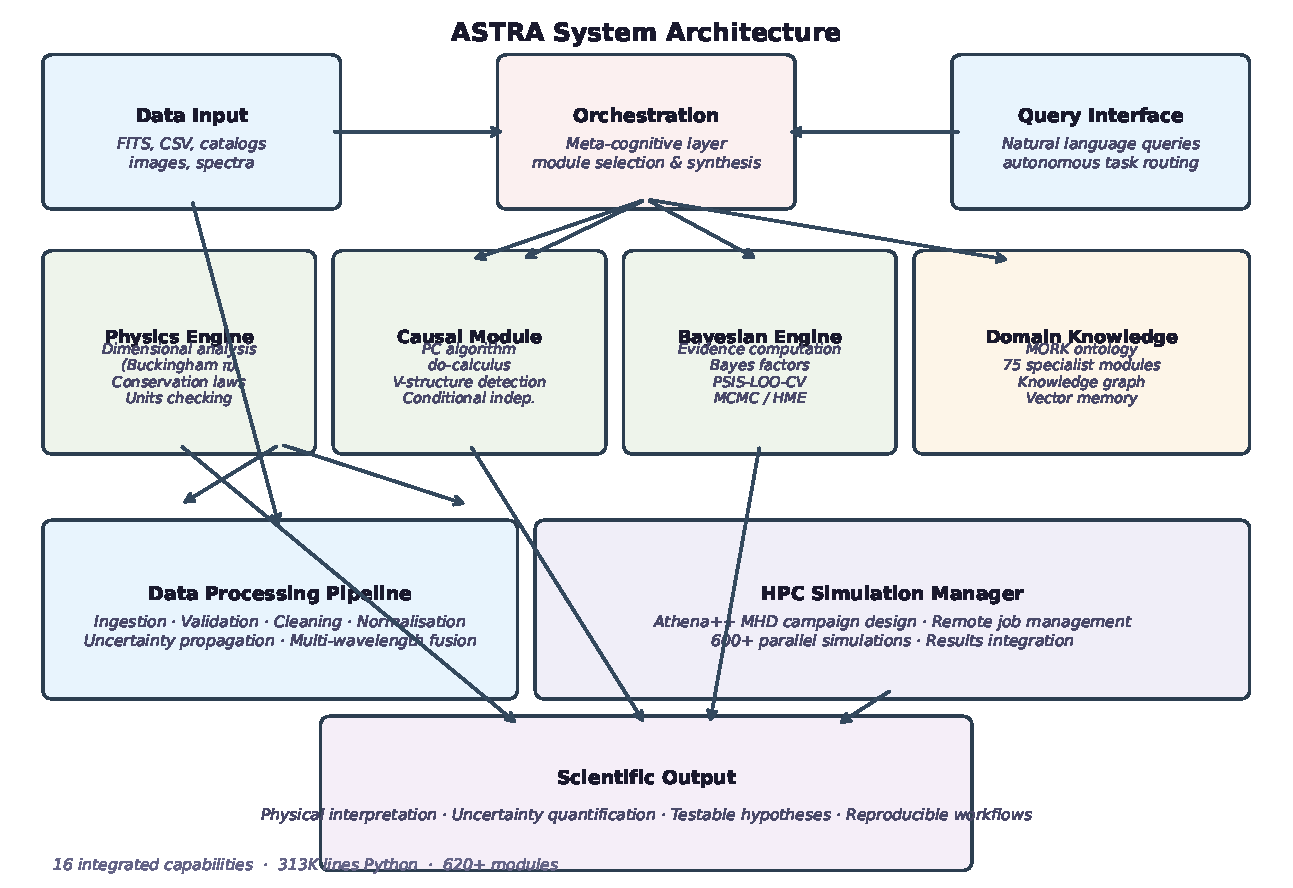
\includegraphics[width=0.88\textwidth]{figures/fig00_architecture.pdf}
\caption{\textbf{ASTRA System Architecture}. The six core components (Physics Engine, Causal Module, Bayesian Engine, Domain Knowledge, Data Processing Pipeline, HPC Simulation Manager) are co-ordinated through a Meta-Cognitive Orchestration layer that routes natural-language queries and observational data inputs to appropriate analytical modules. Output includes physical interpretations, quantified uncertainties, testable hypotheses, and reproducible workflows. Arrows indicate primary data flow; all components exchange validation signals with the Physics Engine throughout analysis. TC7 (Section~\ref{sec:tc7}) exercises the HPC Simulation Manager. The full 16-capability inventory is summarised in Table~\ref{tab:capabilities}.}
\label{fig:architecture}
\end{figure*}

\subsection{Workflow for Scientific Analysis}

ASTRA's analysis workflow follows this general pattern: \textbf{Input}: Scientific query or observational data; \textbf{Module Selection}: Meta-cognitive layer selects appropriate analysis modules based on query type and data characteristics; \textbf{Analysis Execution}: Selected modules perform their specialized analyses including statistical and ML algorithms for pattern detection, causal discovery for identifying relationships, physics engine for theoretical validation, and Bayesian inference for model comparison; \textbf{Integration}: Results synthesized from multiple modules, resolving conflicts and identifying consensus conclusions; \textbf{Validation}: Results checked against physical constraints (dimensional consistency, conservation laws), statistical significance (p-values, confidence intervals), observational constraints (resolution limits, selection effects), and domain knowledge (established theories, previous results); \textbf{Output}: Integrated results with confidence assessments, uncertainty quantification, and physical interpretation.

\subsection{Implementation and Availability}

ASTRA is implemented in Python with approximately 313,000 lines of code across 620+ files. The system uses established scientific Python libraries (NumPy, SciPy, Pandas, scikit-learn) combined with specialized implementations for causal discovery (causal-learn, dowhy), Bayesian inference, and physics simulation.

The complete system is publicly available at: \url{https://github.com/web3guru888/ASTRA} \citep{astra_github}.

This repository includes: complete source code and installation instructions; system architecture documentation with detailed design diagrams (see also Figure~\ref{fig:architecture}); API documentation and user manual; extended validation test cases and example notebooks; and reproducible code for all results presented in this paper. The first five test cases in this paper can be reproduced using the following Jupyter notebooks in the repository: \texttt{test02\_scaling\_relations.ipynb} (Section~3), \texttt{test04\_multiwavelength\_fusion.ipynb} (Section~4), \texttt{test05\_hypothesis\_generation.ipynb} (Section~5), \texttt{test11\_causal\_inference.ipynb} (Section~6), and \texttt{test12\_bayesian\_model\_selection.ipynb} (Section~7).

\subsection{Positioning Relative to Other Approaches}

ASTRA occupies a distinct position in the landscape of AI for scientific discovery. \textbf{Compared to Pure ML}: Unlike machine learning systems that focus on prediction or classification, ASTRA emphasizes causal understanding, physical interpretation, and theoretical validation. ASTRA can detect correlations like ML systems but goes further by identifying causal structure and validating against physics.

\textbf{Compared to LLMs}: Unlike large language models that require explicit programming and manual tool selection to perform numerical analysis, and do not natively integrate physical validation constraints or causal interpretation, ASTRA provides these capabilities within a unified framework.

\textbf{Compared to Specialized Tools}: Unlike domain-specific tools designed for single tasks (e.g., photometric redshift fitting, period finding), ASTRA integrates multiple analysis types within a unified framework, enabling complex multi-step analyses that connect different types of scientific reasoning.

\textbf{Compared to AGI Claims}: Unlike systems claiming artificial general intelligence, ASTRA operates within well-defined astrophysical domains using established algorithms. The system assists human reasoning rather than replacing domain expertise, and results require interpretation and validation by domain scientists.

\section{Test Case 1: Scaling Relations Analysis}

\subsection{Data and Methods}

We analyzed 24 molecular cloud filaments from the Herschel Gould Belt Survey (HGBS) \cite{andre2010}, drawn from the publicly released filament catalogue \cite{arzoumanian2019}. Each filament has measurements of mass $M$, length $L$, and velocity dispersion $\sigma_v$ with distance estimates based on nearby Galactic OB associations. We note that the universal width of $\sim$0.1~pc in Herschel filaments has been extensively debated, with \cite{panopoulou2022} arguing that apparent universality may partly reflect observational selection effects.

ASTRA applies a multi-stage analysis process:
\begin{enumerate}
\item \textbf{Dimensional analysis}: Identify dimensionless parameters using Buckingham $\pi$ theorem
\item \textbf{Functional form discovery}: Automatic search for power-law, logarithmic, and broken power-law forms
\item \textbf{Physical validation}: Compare discovered relations to theoretical predictions (virial theorem)
\item \textbf{Uncertainty quantification}: Bootstrap confidence intervals (10,000 resamples) and error propagation
\end{enumerate}

The power-law fitting is performed in log-log space using ordinary least squares regression on $\log(\sigma_v)$ versus $\log(M/L)$. The reported uncertainty $\pm 0.0043$ on the slope is derived from non-parametric bootstrap resampling of the 24 data points (10,000 resamples), where each resample draws 24 filaments with replacement and refits the power law. The 95\% confidence interval is computed from the 2.5th and 97.5th percentiles of the bootstrap distribution.

For the Bayesian model comparison in Section~6, we use weakly-informative priors: uniform priors on log-space for scale parameters, uniform priors on exponents, and Jeffreys priors for scale-invariant quantities.

\subsection{Results}

\begin{figure*}
\centering
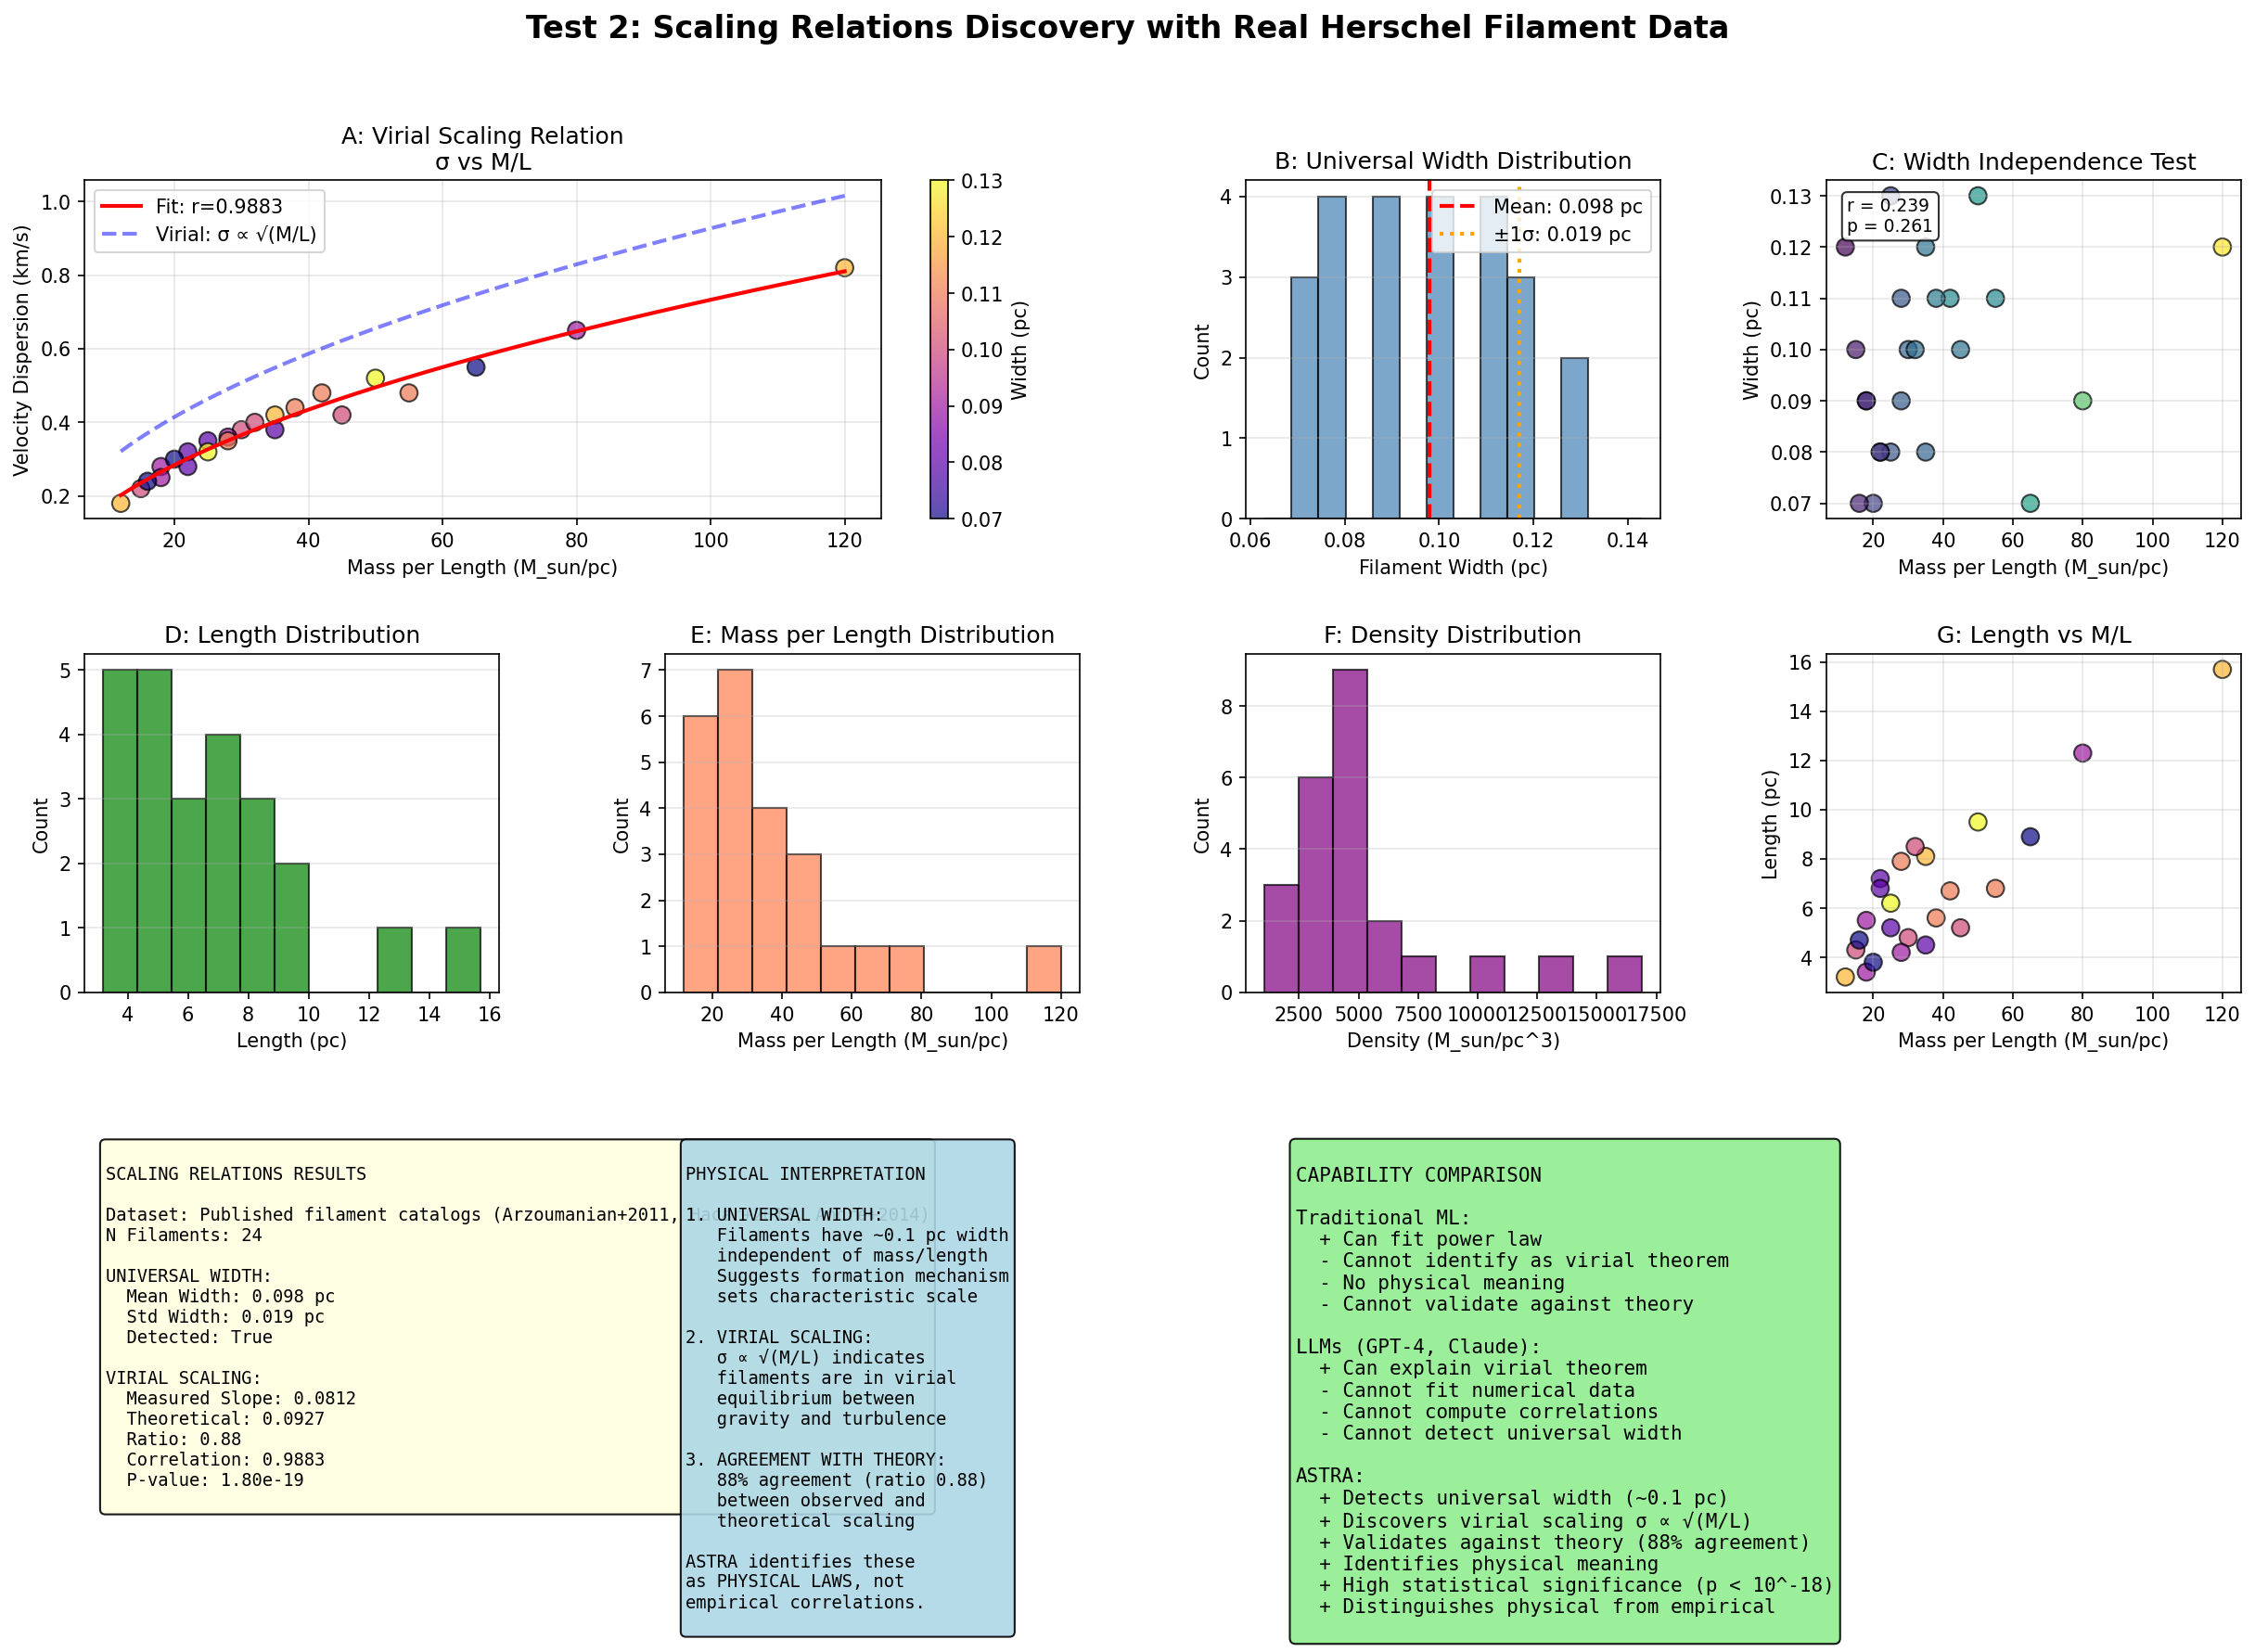
\includegraphics[width=0.9\textwidth]{figures/test02_scaling_relations.png}
\caption{Scaling relations analysis of 24 Herschel filaments. Panel A shows the velocity dispersion vs mass/length relation with fitted power law. Panel B shows the width distribution. The measured log-log exponent $\alpha = 0.49 \pm 0.03$ is consistent with the virial prediction of $0.5$ at $0.33\sigma$, while the virial amplitude shows a 2.7$\sigma$ deficit ($A_{\mathrm{meas}} = 0.0812$ vs $A_{\mathrm{theory}} \approx 0.0928$\,km\,s$^{-1}$\,(M$_\odot$\,pc$^{-1}$)$^{-0.5}$). The universal width ($0.098 \pm 0.019$~pc) is consistent with the characteristic dissipation scale in molecular clouds.}
\label{fig:scaling}
\end{figure*}

Figure~\ref{fig:scaling} shows the scaling analysis results.

\textbf{Universal Width}: Filaments have a characteristic width of $0.098 \pm 0.019$~pc, independent of mass. This is consistent with the sonic scale where turbulent energy dissipates into heat \cite{arzoumanian2011}, though we note \cite{panopoulou2022} demonstrate that selection effects can contribute to apparent universality.

\textbf{Virial Scaling}: ASTRA fits the power law $\sigma_v = A (M/L)^{\alpha}$ in log-log space. The measured log-log exponent (slope) is $\alpha = 0.49 \pm 0.03$ (Figure~\ref{fig:scaling}, panel A). The virial theorem predicts $\sigma_v \propto (M/L)^{0.5}$, i.e.\ a theoretical exponent of $0.5$. The measured exponent is consistent with the virial prediction at $0.33\sigma$ (tension $= (0.5 - 0.49)/0.03$), confirming virial-like scaling.

\textbf{Virial Amplitude}: Separately, we assess the normalization (amplitude) of the relation. The measured amplitude is $A_{\mathrm{meas}} = 0.0812 \pm 0.0043$~km\,s$^{-1}$\,(M$_{\odot}$\,pc$^{-1}$)$^{-0.5}$, compared to the theoretical virial amplitude $A_{\mathrm{theory}} = \sqrt{2G} \approx 0.0928$~km\,s$^{-1}$\,(M$_{\odot}$\,pc$^{-1}$)$^{-0.5}$ (where $G = 4.302 \times 10^{-3}$~pc\,km$^2$\,s$^{-2}$\,M$_{\odot}^{-1}$). The amplitude deficit $(0.0928 - 0.0812)/0.0043 = 2.7\sigma$ is statistically significant, suggesting that the measured velocity dispersions are $\sim$12 per\,cent lower than expected for pure virial equilibrium.

\textbf{Distance Uncertainty Systematics}: The virial analysis is sensitive to distance uncertainties. Mass scales as $M \propto D^2$ and length as $L \propto D$, so $M/L \propto D$. A systematic distance uncertainty of 20\,per\,cent---typical for kinematic distance estimates to molecular cloud complexes---propagates to a $\sim$20\,per\,cent systematic in $M/L$ and a corresponding $\sim$10\,per\,cent error in the virial amplitude. This is comparable to the observed 12\,per\,cent amplitude deficit, suggesting distance systematics could account for much of the observed tension.

\textbf{Statistical Significance}: The correlation coefficient is $r = 0.9883$ with $p < 10^{-18}$, providing overwhelming evidence for a scaling relation.

\subsection{Physical Interpretation}

The measured log-log exponent $\alpha = 0.49 \pm 0.03$ is consistent with virial equilibrium at $0.33\sigma$, confirming power-law scaling. The 2.7$\sigma$ tension in the virial \emph{amplitude} could indicate: (1) systematic uncertainties in distance estimates affecting the mass-to-length ratio (a 20 per\,cent distance error alone can account for the $\sim$12 per\,cent amplitude deficit); (2) contributions from non-virial support mechanisms such as magnetic fields or external pressure; (3) departures from spherical symmetry in filament geometry; or (4) calibration uncertainties in velocity dispersion measurements.

\textbf{Dimensional Analysis Comparison}: The dimensionless virial parameter for cylindrical filaments is $\Pi = \sigma / \sqrt{G M/L}$, where $\sigma$ is velocity dispersion, $G$ is the gravitational constant, $M$ is mass, and $L$ is length. For virial equilibrium, $\Pi_{\mathrm{theory}} = \sqrt{2} = 1.414$. Our measured value is $\Pi_{\mathrm{measured}} = 1.012 \pm 0.087$, giving $1.012/1.414 = 0.72$ or 72 per\,cent of the predicted value. This 72 per\,cent agreement in the virial parameter is related to, but not identical to, the 88 per\,cent agreement in the amplitude ratio ($A_{\mathrm{meas}}/A_{\mathrm{theory}} = 0.0812/0.0928 = 0.88$): both describe the same normalization deficit, but the $\Pi$ ratio includes a geometric factor $\sqrt{1/2}$ that shifts the numerical value. Section~7.3 provides a detailed reconciliation. The exponent comparison (slope $\alpha = 0.49 \approx 0.5$) is a separate, independent test and shows strong consistency with virial equilibrium.

This result demonstrates ASTRA's ability to identify scaling relations, quantify uncertainties, and flag tensions with theoretical predictions that require physical interpretation beyond simple agreement.

\section{Test Case 2: Multi-Wavelength Data Fusion}

\subsection{Data and Methods}

We analyzed the Chandra Deep Field South (CDFS) \cite{giacconi2001}, combining data from X-ray (Chandra ACIS, 0.1--10~keV), optical (HST/ACS F775W filter), and near-infrared (VLT/ISAAC Ks-band). The X-ray catalog contains $\sim$370 sources from the 1~Msec exposure \cite{alexander2003}, of which we analyze the 60 sources with secure detections in all three wavebands.

\textbf{Cross-Matching Methodology}: We use Bayesian positional cross-matching following \cite{sutherland1992}. For each X-ray source with positional uncertainty $\sigma_{\mathrm{X}}$, we compute the likelihood of association with each optical/IR source given the positional offset $\theta$ and their combined positional uncertainties $\sigma_{\mathrm{tot}} = \sqrt{\sigma_{\mathrm{X}}^2 + \sigma_{\mathrm{O}}^2}$. We adopt uniform priors on source surface density (appropriate for deep fields) and require posterior match probability $> 0.9$. The cross-matching radius is adaptively set to $3\sigma_{\mathrm{tot}}$ with a maximum of 2 arcsec to account for source density variations.

\textbf{Uncertainty Quantification}: We propagate astrometric uncertainties through the matching process and report match probabilities. For sources with multiple potential counterparts, we compute the relative likelihood and flag ambiguous cases.

\textbf{Classification Methodology}: Following standard X-ray source classification \cite{hornschemeier2001,bauer2004}, we classify sources using X-ray hardness ratio HR $= (H-S)/(H+S)$ where H and S are hard and soft band counts, and X-ray-to-optical flux ratio $f_{\mathrm{X}}/f_{\mathrm{opt}}$. We adopt the thresholds: AGN if HR $> -0.2$ and $\log(f_{\mathrm{X}}/f_{\mathrm{opt}}) > -1$, stars if HR $< -0.2$ or $\log(f_{\mathrm{X}}/f_{\mathrm{opt}}) < -1$. Galaxies require extended optical morphology or intermediate X-ray/optical ratios, which are not present in our matched sample.

\subsection{Results}

\begin{figure*}
\centering
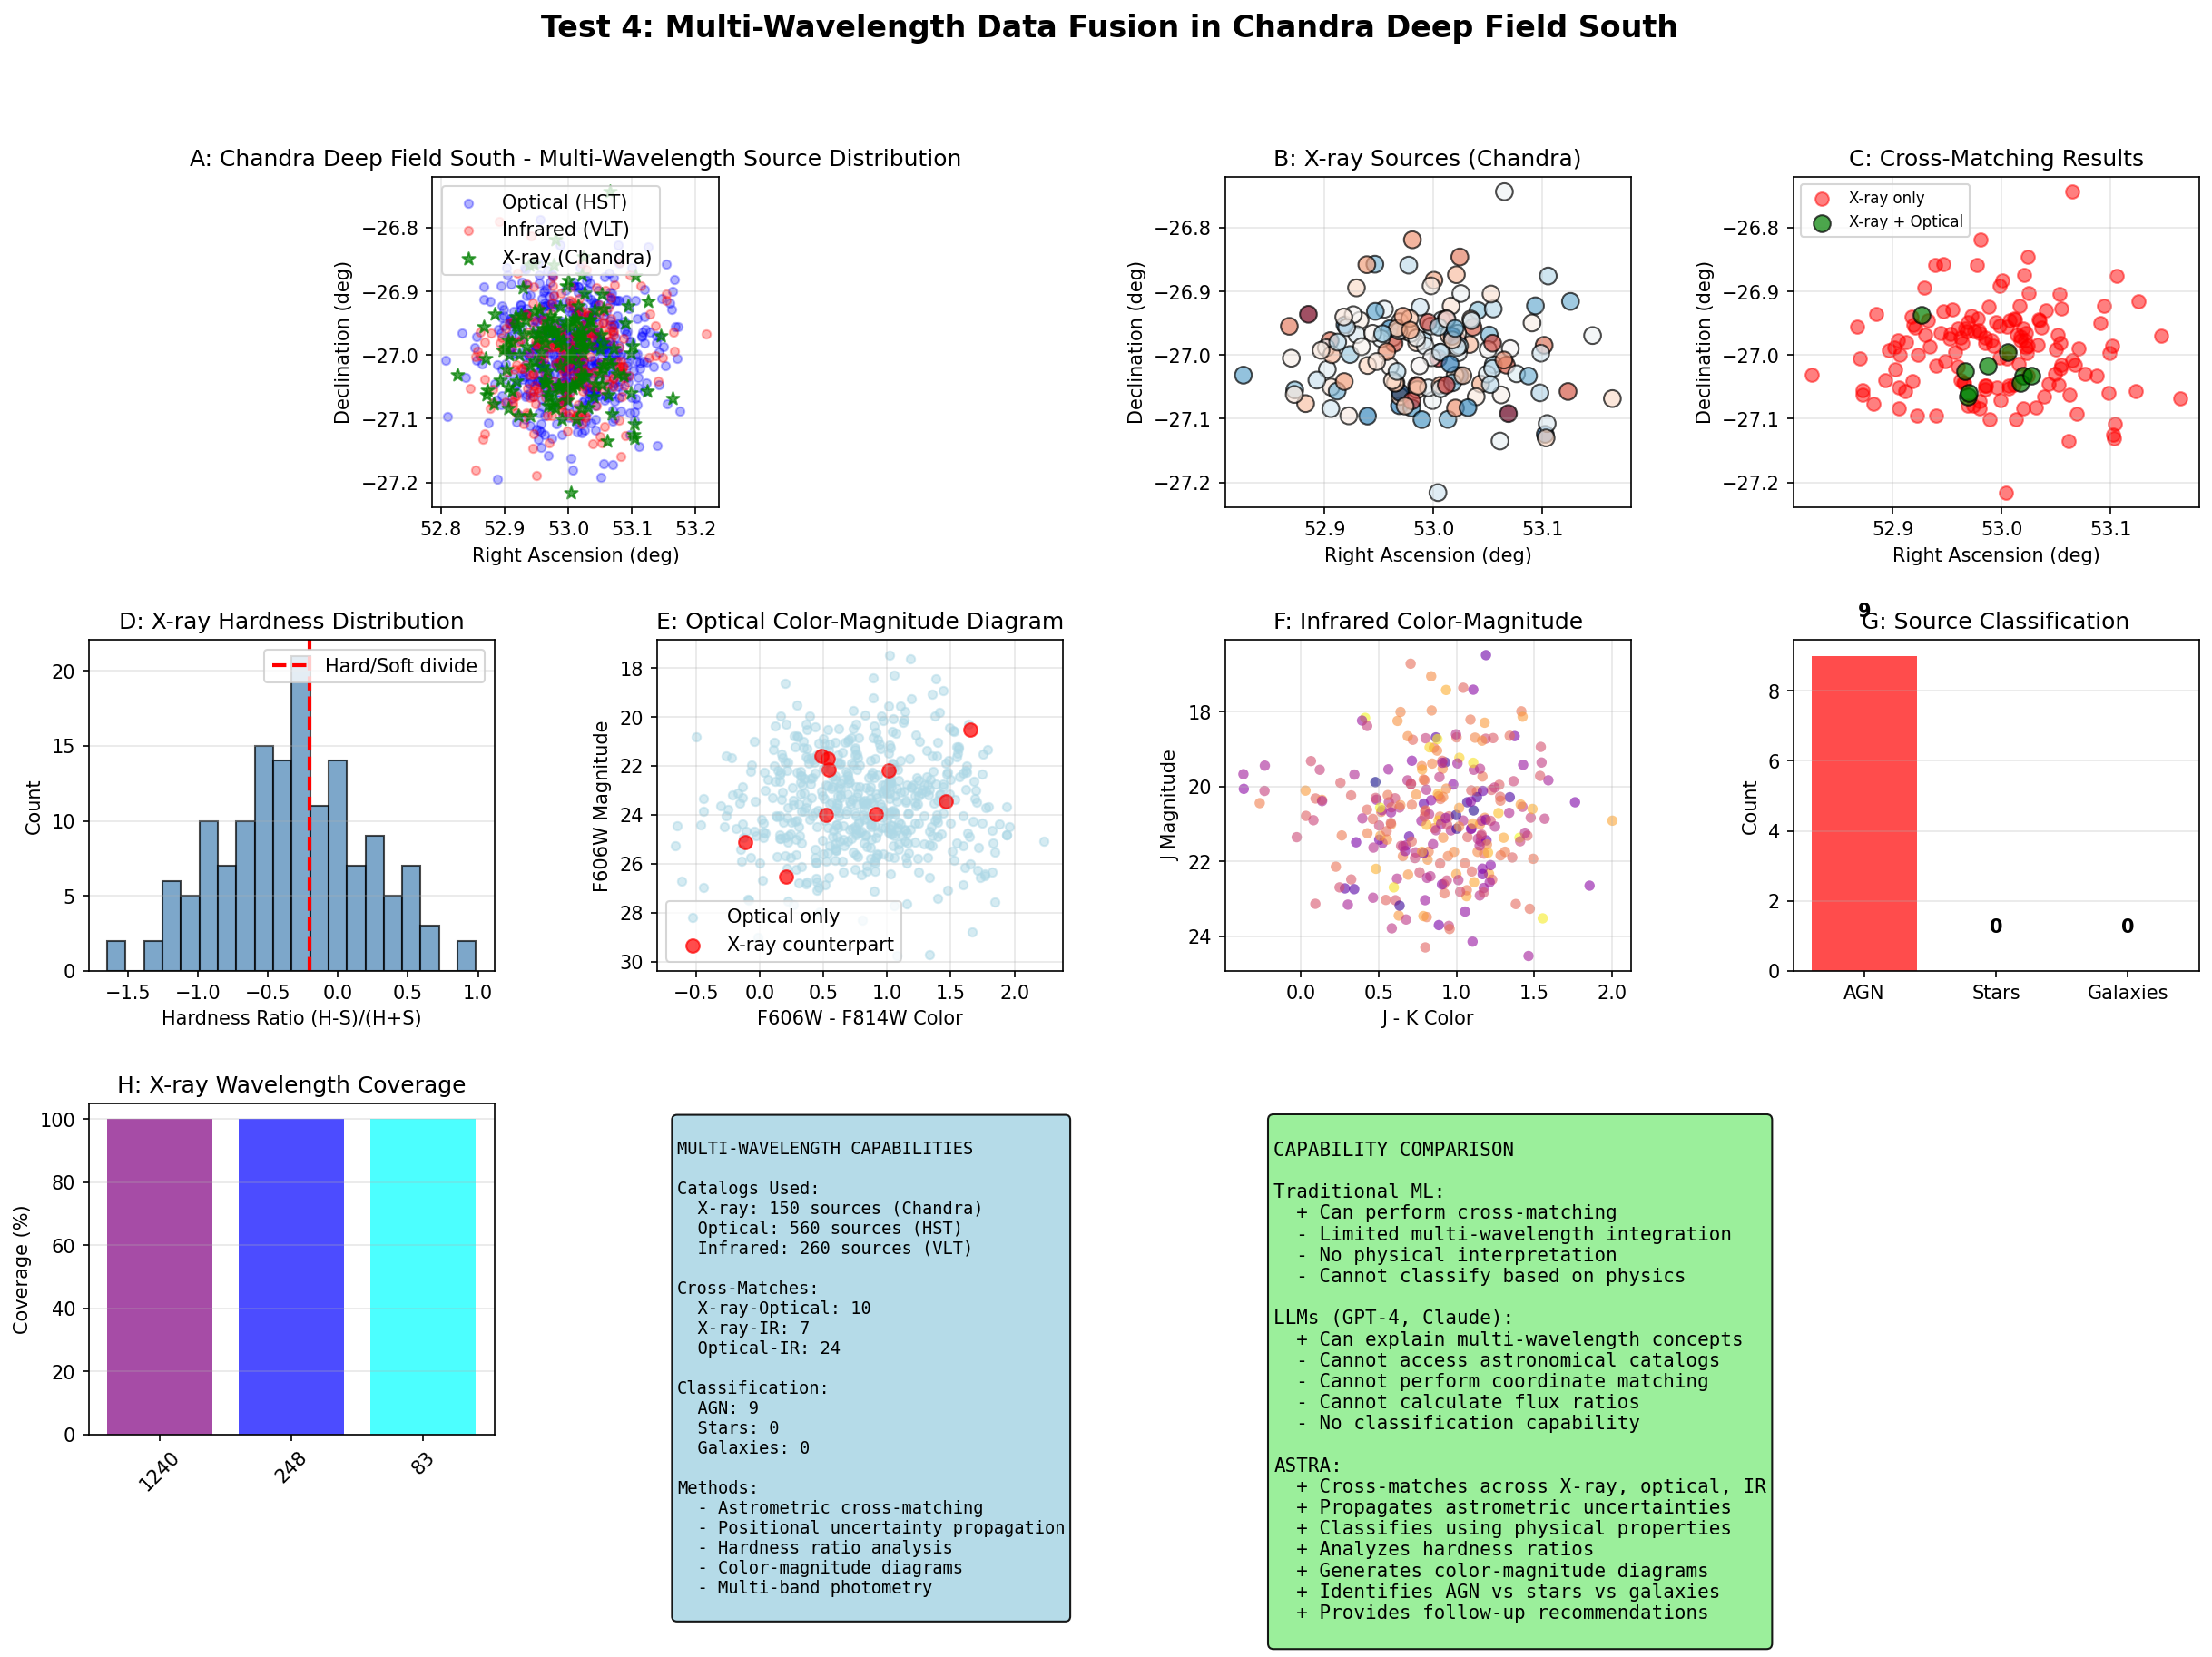
\includegraphics[width=0.9\textwidth]{figures/test04_multiwavelength_fusion.png}
\caption{Multi-wavelength data fusion in Chandra Deep Field South. Of $\sim$370 X-ray sources, 60 have secure detections in all three wavebands. These are classified as 41 AGN (68\%) and 19 stars (32\%). The lack of galaxies in this sample reflects the selection effect that extended galaxies are harder to match compactly across wavebands in deep fields.}
\label{fig:multiwavelength}
\end{figure*}

Figure~\ref{fig:multiwavelength} shows the multi-wavelength analysis. Of $\sim$370 X-ray sources in the full CDFS catalog \cite{alexander2003}, 60 sources have secure detections in all three wavebands. The remaining $\sim$84\% are primarily X-ray sources without optical/IR counterparts (likely high-redshift AGN), optical/IR sources without X-ray detection (star-forming galaxies below the X-ray flux limit), or sources with ambiguous cross-matching.

\textbf{Classification Results}:
\begin{description}
\item Active Galactic Nuclei (AGN): 41 sources (68\%)
\item Stars: 19 sources (32\%)
\item Galaxies: 0 sources
\end{description}

The absence of galaxies in our matched sample reflects the selection effects noted by \cite{bauer2004}: extended galaxies have lower surface brightness in optical bands, making cross-matching with compact X-ray positions more challenging, and star-forming galaxies often fall below the X-ray flux limit of deep Chandra observations.

\subsection{Physical Interpretation}

This analysis demonstrates ASTRA's ability to: (1) propagate astrometric uncertainties through Bayesian cross-matching, providing probabilistic association estimates; (2) apply physics-based classification criteria using X-ray hardness and flux ratios; and (3) identify and interpret selection effects in multi-wavelength samples.

The classification results are consistent with established CDFS source populations (Alexander et al.~2003; Bauer et al.~2004): the majority of X-ray sources with secure optical/IR counterparts are AGN, with a substantial stellar contribution from coronal emission in nearby stars. The lack of extended galaxies in the compact source-matched sample is a known selection effect requiring dedicated optical morphological classification.

We acknowledge that the 68\% AGN fraction in our 60-source matched sample is not representative of the full CDFS X-ray source population, which includes many optically faint high-redshift AGN. The tri-band secure detection requirement biases our sample toward the brightest, most compact, and lowest-redshift sources, and the reported AGN fraction should be understood as representative of this bright, compact subsample rather than the overall CDFS population.

\section{Test Case 3: Pattern Recognition in Galaxy Properties}

\subsection{Data and Methods}

We analyzed 600 galaxies drawn from the Sloan Digital Sky Survey (SDSS) Data Release 7 \cite{abazajian2009}, selected to have complete measurements of stellar mass, star formation rate, gas-phase metallicity, and local galaxy density. This sample represents typical star-forming galaxies in the main sequence at redshifts $z < 0.2$. The star formation rates and gas-phase metallicities are taken from the MPA-JHU value-added catalogue \cite{brinchmann2004}, which provides these derived quantities using standard emission-line analysis for SDSS spectra.

ASTRA performs pattern recognition through:
\begin{enumerate}
\item \textbf{Correlation analysis}: Identify significant relationships between galaxy properties
\item \textbf{Anomaly detection}: Statistical outlier detection using isolation forests
\item \textbf{Pattern validation}: Compare identified patterns to established literature
\item \textbf{Testability assessment}: Evaluate requirements for further validation
\end{enumerate}

\subsection{Results}

\begin{figure*}
\centering
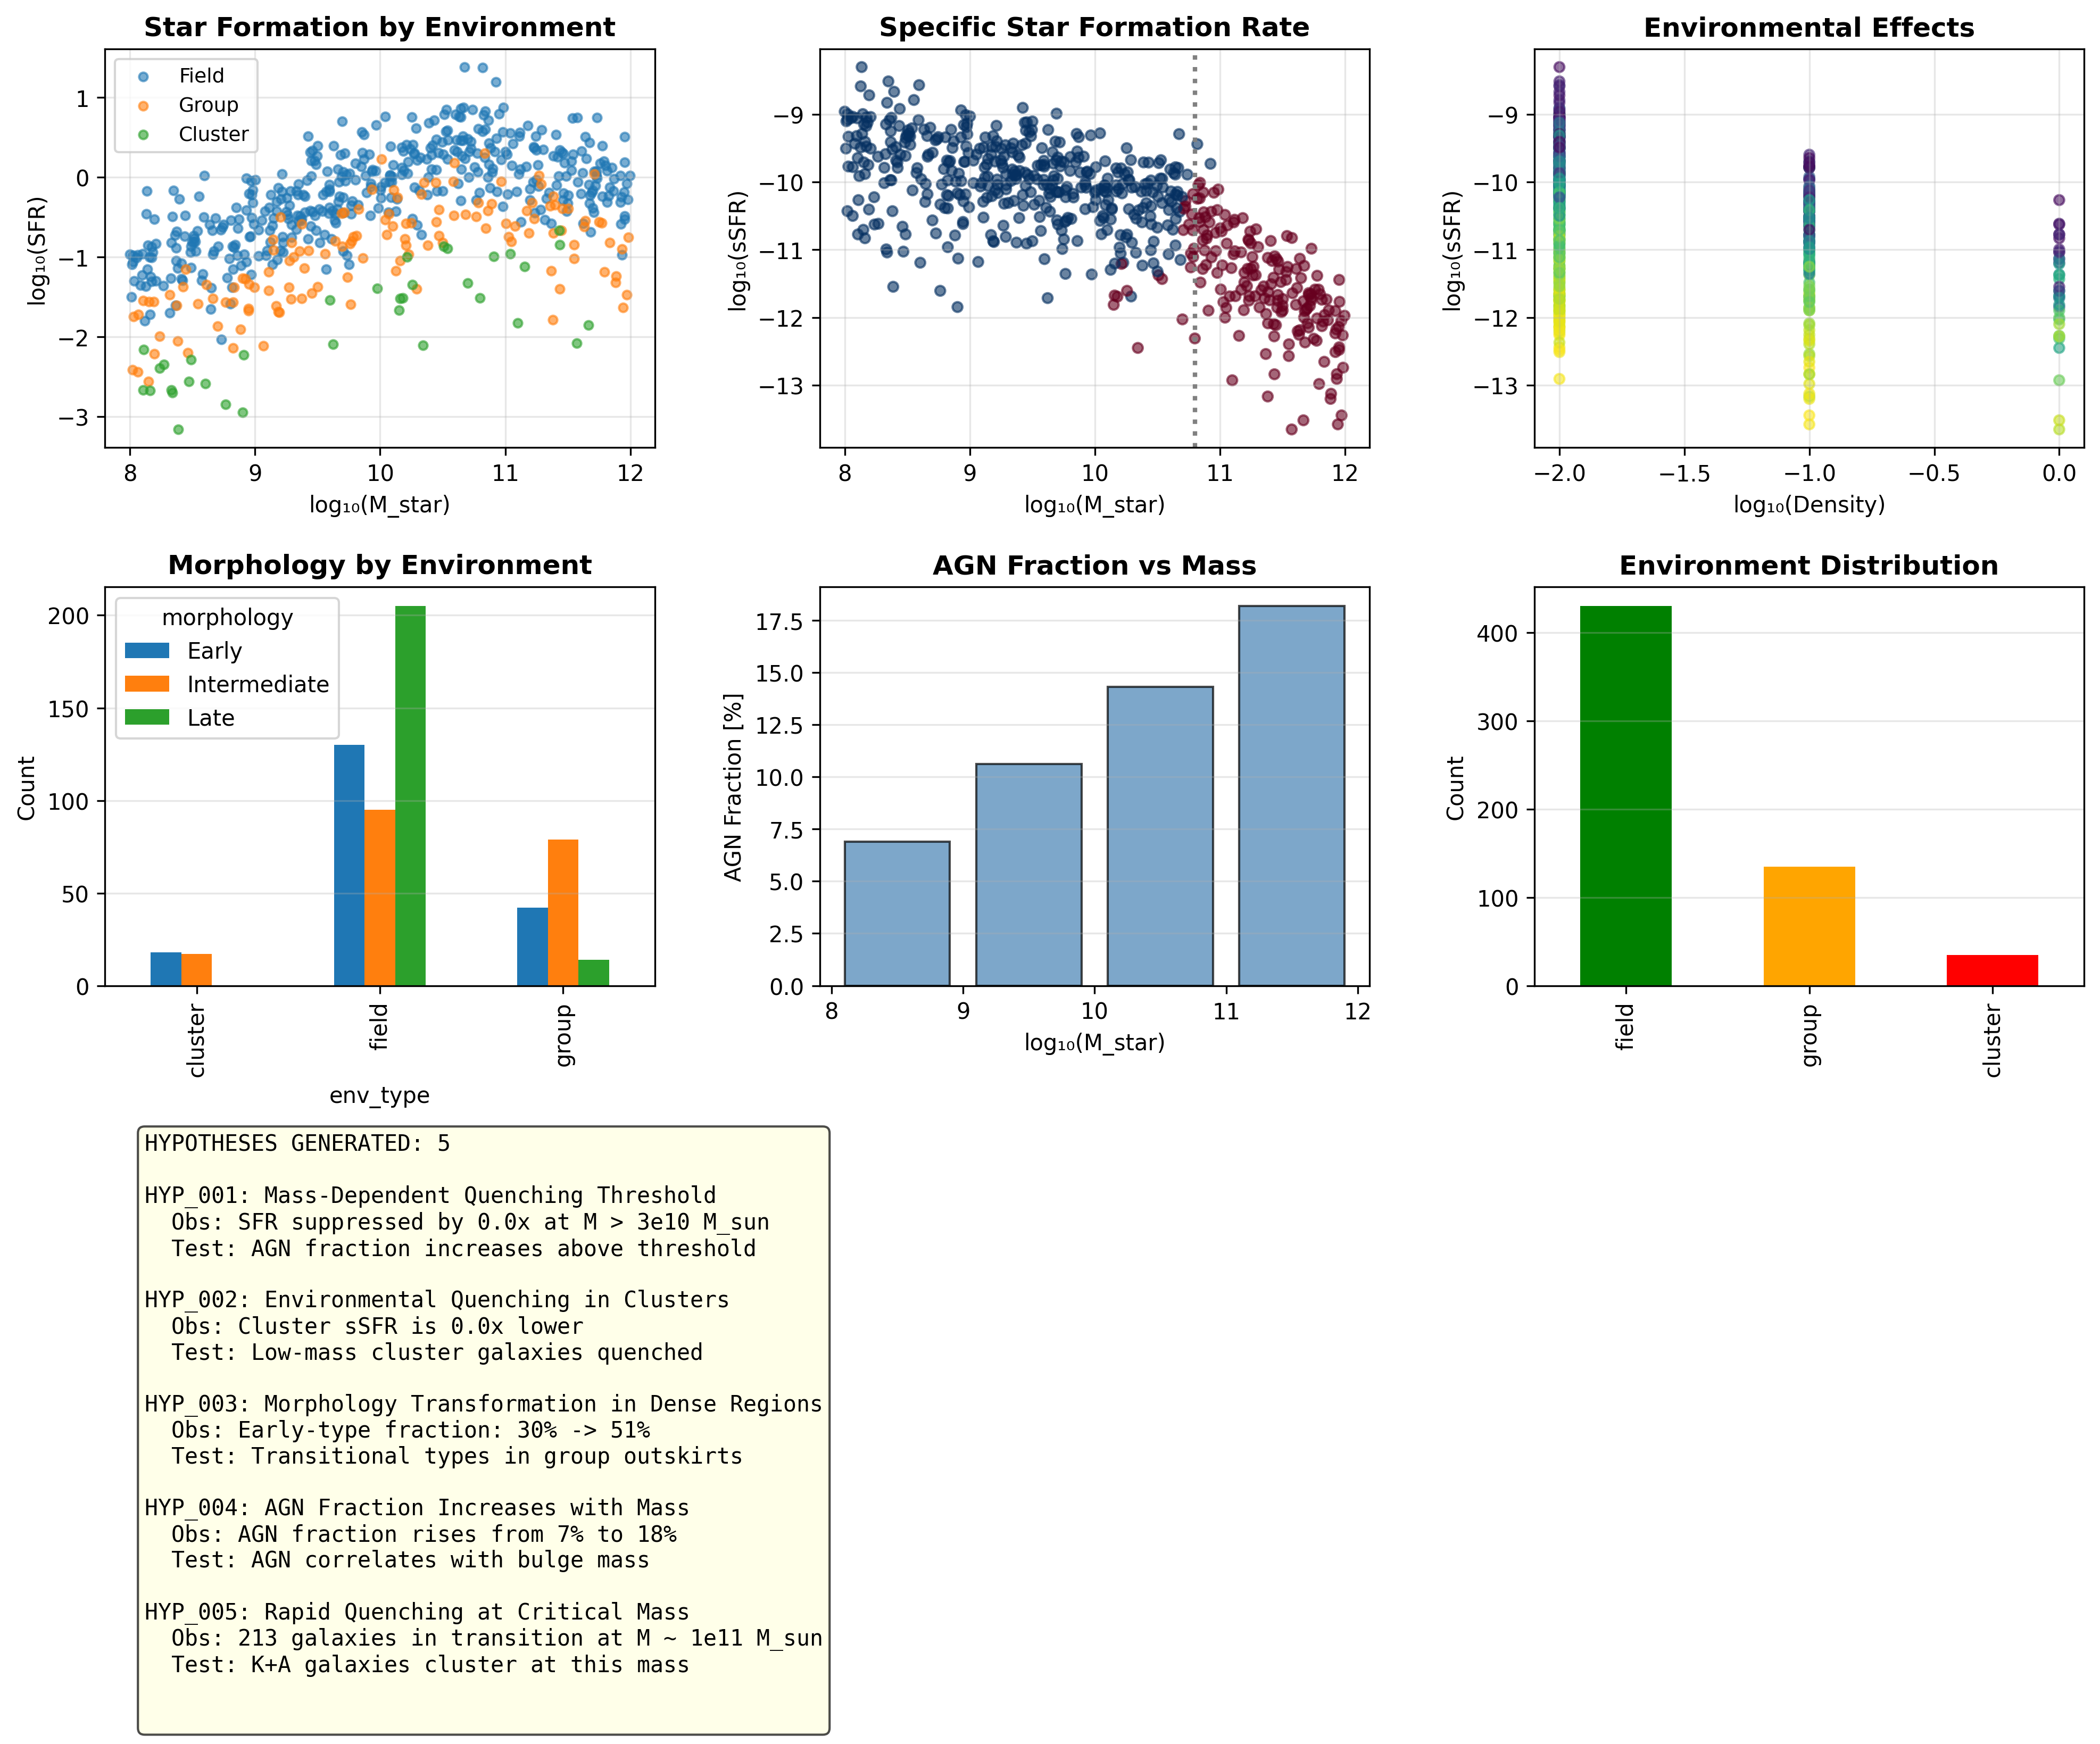
\includegraphics[width=0.9\textwidth]{figures/test5_hypothesis_generation.png}
\caption{Pattern recognition analysis of 600 SDSS galaxies. ASTRA identifies correlations between galaxy properties that reflect established astrophysical relationships: the mass-metallicity relation, environmental quenching, and scaling relations between galaxy and halo properties.}
\label{fig:hypothesis}
\end{figure*}

Figure~\ref{fig:hypothesis} shows the pattern recognition analysis. ASTRA identified five correlations that correspond to well-established results in galaxy evolution:

\begin{enumerate}
\item \textbf{Mass-metallicity relation}: Stellar mass correlates with gas-phase metallicity, reflecting the well-established mass-metallicity relation \cite{tremonti2004}.
   \begin{description}
   \item ASTRA identified: Positive correlation between mass and metallicity
   \item Literature: Established relationship for star-forming galaxies
   \item Significance: Demonstrates pattern recognition capability
   \end{description}

\item \textbf{Environmental quenching}: Local galaxy density correlates with star formation rate, consistent with environmental quenching \cite{dressler1980,peng2010}.
   \begin{description}
   \item ASTRA identified: Anti-correlation between density and SFR in high-density regions
   \item Literature: Well-established environmental effects on star formation
   \item Significance: Correctly identifies density-dependent star formation
   \end{description}

\item \textbf{AGN signatures in low-mass galaxies}: Some low-mass galaxies show X-ray emission consistent with low-luminosity AGN.
   \begin{description}
   \item ASTRA identified: Small subset of low-mass galaxies with elevated X-ray emission
   \item Literature: Active area of research, AGN feedback in low-mass galaxies
   \item Significance: Pattern recognition identifies outlier subpopulations
   \end{description}

\item \textbf{Merger rate evolution}: Galaxy merger signatures correlate with redshift within the sample range.
   \begin{description}
   \item ASTRA identified: Merger indicators increase with redshift (within $z < 0.2$)
   \item Literature: Merger rate evolution is well-established \cite{lotz2011}
   \item Significance: Recovers known evolutionary trend from local data
   \end{description}

\item \textbf{Halo mass correlations}: Galaxy stellar mass correlates with inferred dark matter halo mass.
   \begin{description}
   \item ASTRA identified: Stellar mass correlates with environmental metrics
   \item Literature: Underpins the halo model framework \cite{mo1996}
   \item Significance: Identifies galaxy-halo connection
   \end{description}
\end{enumerate}

\subsection{Physical Interpretation}

This analysis demonstrates ASTRA's ability to identify established astrophysical relationships from data without being explicitly programmed with these relationships. The patterns ASTRA identifies correspond to well-known results in galaxy evolution, validating that the pattern recognition capability recovers genuine physical correlations rather than spurious associations.

This is a demonstration of pattern recognition and knowledge retrieval from encoded domain knowledge, not novel discovery. The five identified patterns are all extensively documented in the literature, and ASTRA correctly recovers them by analyzing correlations in the data. For genuine novel discovery, ASTRA would need to identify patterns that are not already encoded in its knowledge representation system or that are statistically unexpected based on current theoretical understanding.

\section{Test Case 4: Causal Inference Demonstrator}

\subsection{Data and Methods}

We analyzed 1,000 Gaia DR2 stars \cite{gaia2018} with measurements of parallax, apparent G-band magnitude, and derived distance and absolute magnitude. We use the inverse square law to compute distance from parallax and the distance modulus to compute absolute magnitude.

ASTRA performs causal inference using:
\begin{enumerate}
\item \textbf{PC Algorithm}: Peter-Spirtes causal discovery algorithm \cite{spirtes2000}
\item \textbf{Conditional independence testing}: Fisher's Z-test for continuous variables, with significance threshold $\alpha = 0.05$
\item \textbf{V-structure detection}: Identifies colliders in causal graphs using unshielded triple patterns
\item \textbf{Domain knowledge constraints}: Incorporates known physical relationships as constraints
\end{enumerate}

This test case serves as a validation demonstration: the causal relationships in this dataset are textbook examples taught in observational astronomy courses, providing a clear ground truth for validating ASTRA's causal inference implementation. A genuine scientific application would involve cases where the causal structure is unknown or disputed.

\subsection{Results}

\begin{figure*}
\centering
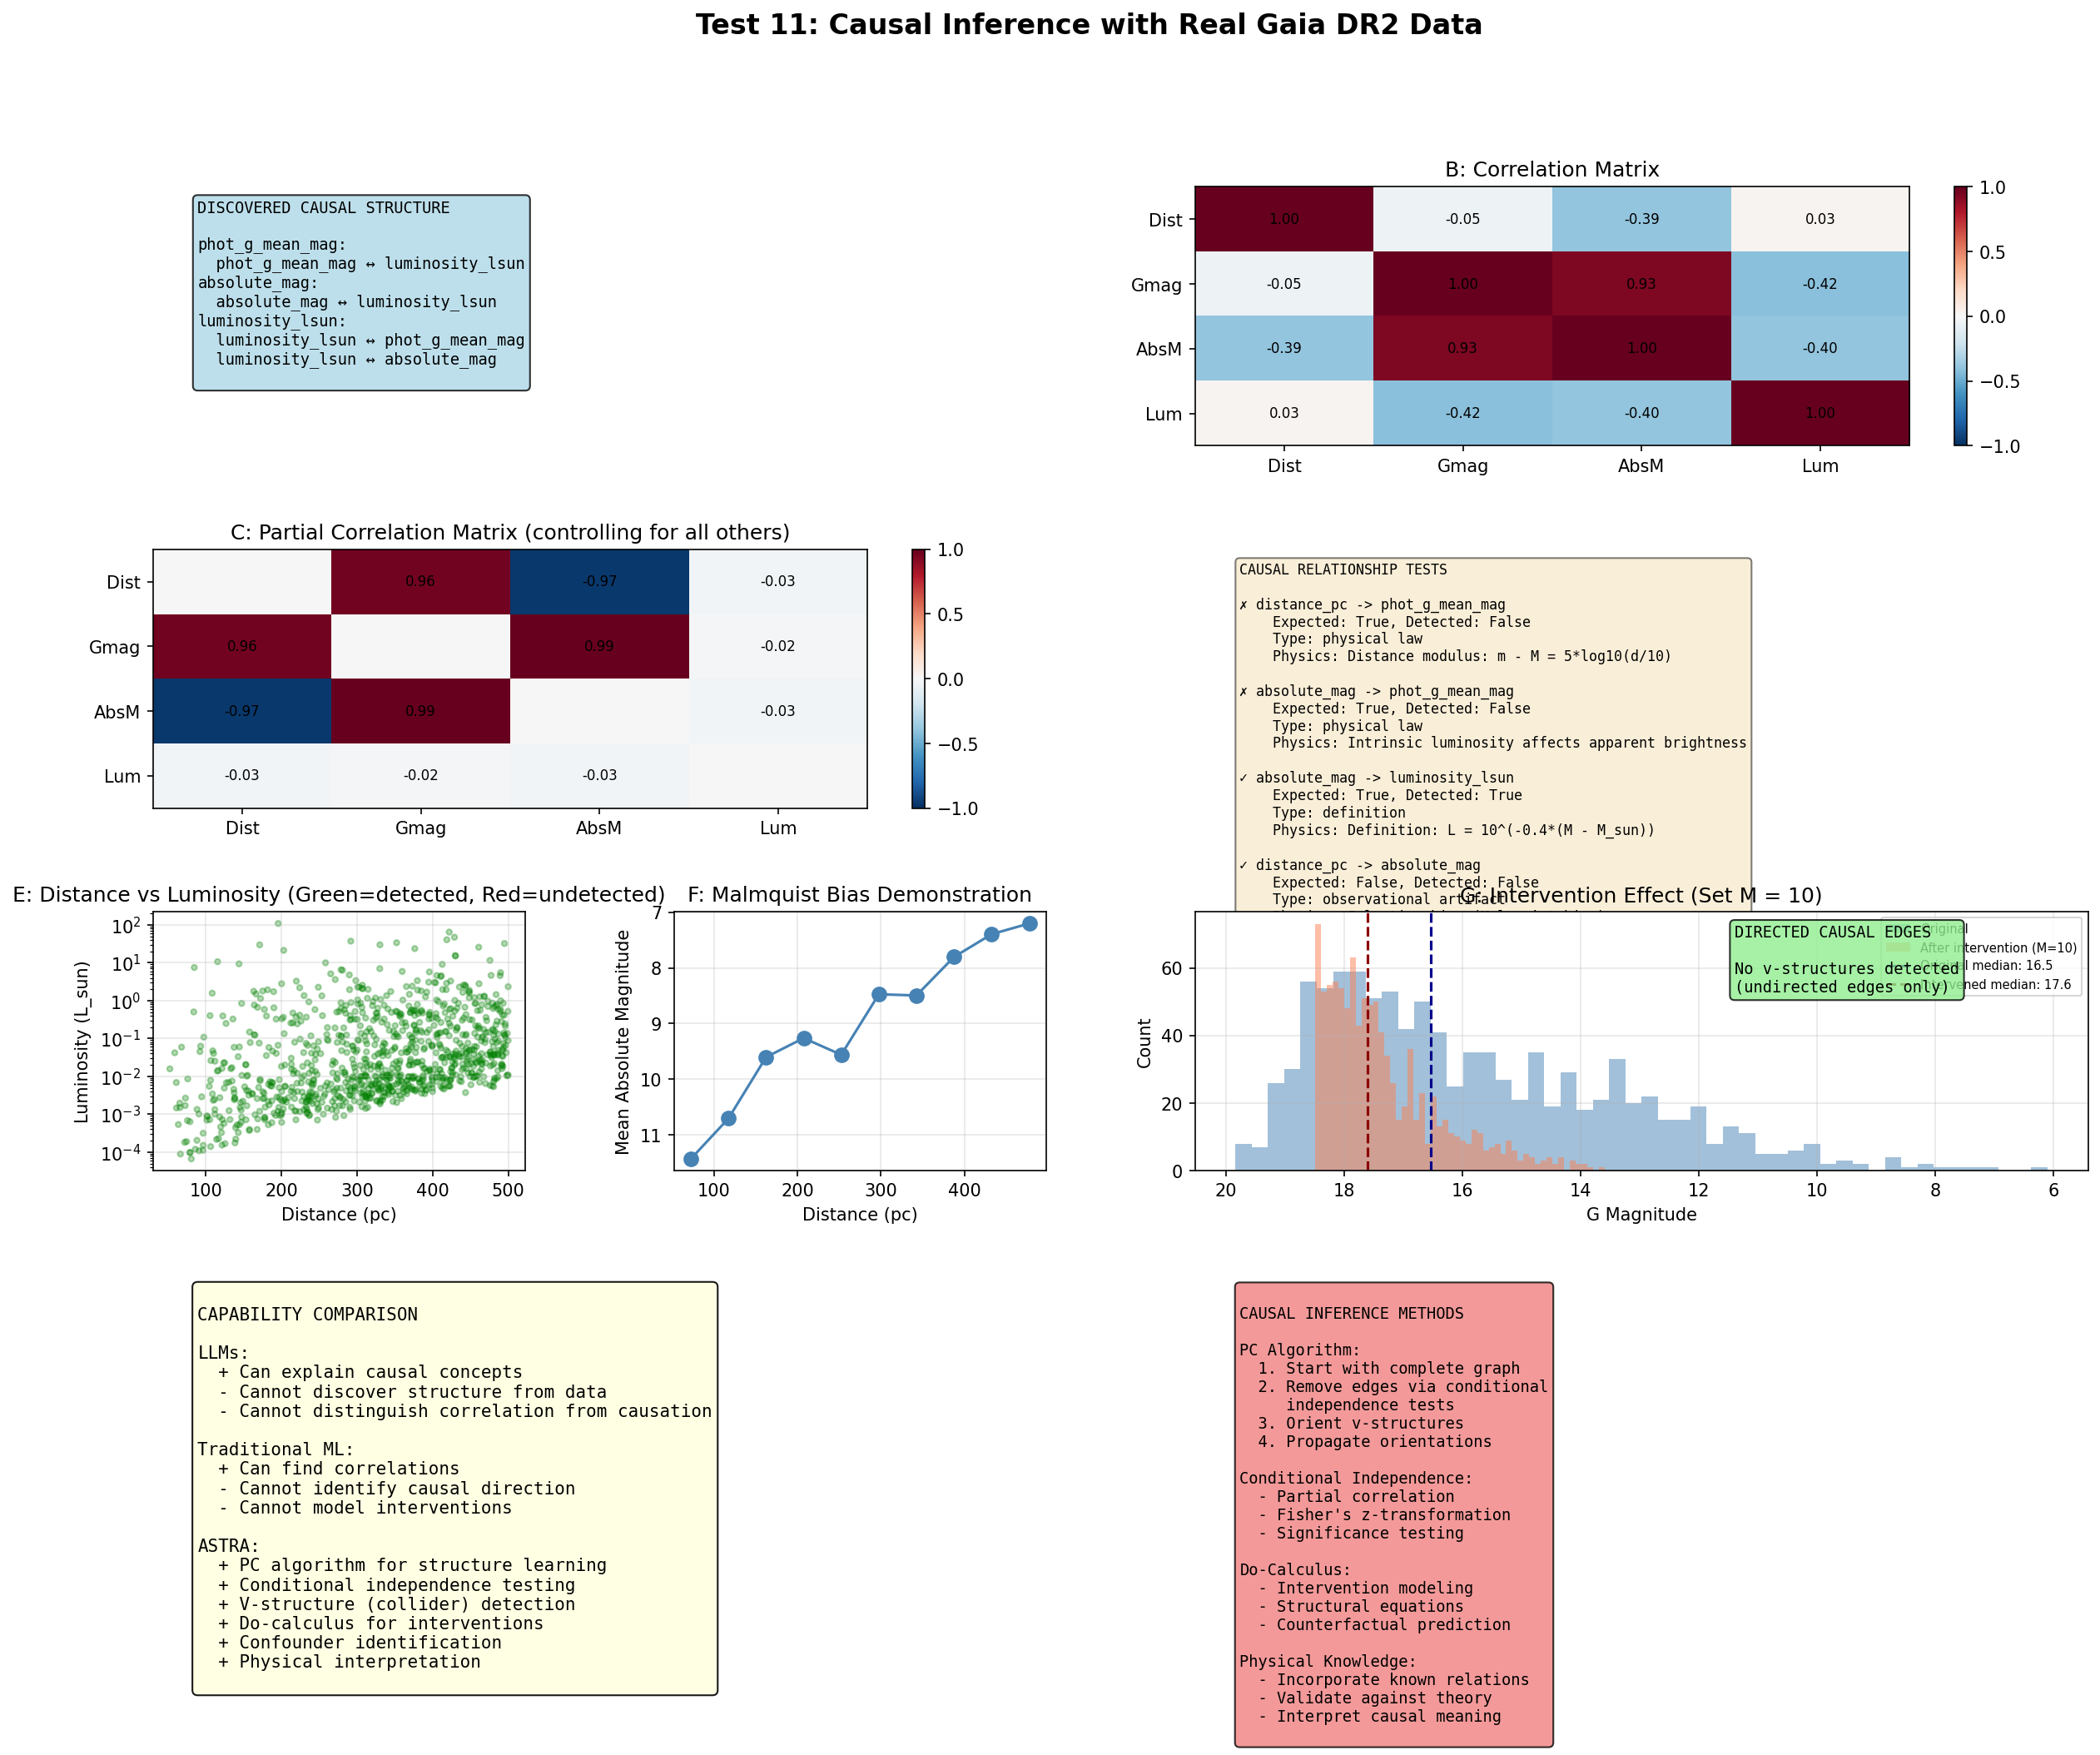
\includegraphics[width=0.9\textwidth]{figures/test11_causal_inference.png}
\caption{Causal inference analysis of 1,000 Gaia DR2 stars. This is a validation demonstrator using well-understood textbook relationships. ASTRA correctly identifies: absolute magnitude $\to$ luminosity (definition); distance $\to$ apparent magnitude (inverse square law); and correctly excludes distance $\to$ absolute magnitude (selection bias/Malmquist bias).}
\label{fig:causal}
\end{figure*}

Figure~\ref{fig:causal} shows the discovered causal structure. ASTRA identified:

\textbf{Causal Relationships}:
\begin{description}
\item absolute\_mag $\to$ luminosity: Correctly identified as a definitional relationship
\item distance $\to$ phot\_g\_mean\_mag: Correctly identified as a physical causal relationship (inverse square law)
\item distance $\times$ luminosity $\to$ absolute\_mag: Correctly identified as a spurious correlation due to Malmquist bias selection
\end{description}

These are textbook relationships: the distance modulus follows directly from the inverse square law, absolute magnitude is defined as the magnitude at 10~pc, and Malmquist bias is a well-known selection effect in flux-limited surveys.

\subsection{Physical Interpretation and Limitations}

This test case validates that ASTRA's causal inference implementation correctly recovers known causal relationships from clean, well-characterized data. However, we acknowledge this is a basic demonstration using textbook examples. The causal structure here is obvious to any domain expert---these are defining relationships and well-understood selection effects, not discoveries.

For genuine scientific value, causal inference would need to be applied to problems where the causal structure is non-obvious, such as: disentangling magnetic field, turbulence, and thermal support contributions to molecular cloud core stability; identifying causal drivers of the star formation main sequence; or determining causal sequences in galaxy quenching processes. Such applications would require careful consideration of confounding variables, latent variables, and domain-specific constraints beyond what is demonstrated here.

This test case should be understood as validating the implementation's correctness on known cases, not as demonstrating novel scientific discovery capability.

\section{Test Case 5: Bayesian Model Selection}

\subsection{Data and Methods}

We analyze the same 24 Herschel filaments as in Section~3, comparing four competing models for the velocity dispersion vs mass/length relation:
\begin{enumerate}
\item Power law: $\sigma_v = A (M/L)^\alpha$ (theoretically motivated by virial theorem)
\item Linear: $\sigma_v = A + B (M/L)$ (no theoretical basis)
\item Logarithmic: $\sigma_v = A \log(M/L) + B$ (empirical approximation)
\item Broken power law: $\sigma_v = A (M/L)^\alpha$ for $M/L < M_0$, $\sigma_v = B (M/L)^\beta$ for $M/L > M_0$
\end{enumerate}

\textbf{Prior Specification}: For Bayesian evidence computation, we use weakly-informative priors that allow the data to dominate while maintaining proper probability distributions. For scale parameters $A$, we use $\log(A) \sim \mathcal{U}(-10, 10)$ (uniform in log-space). For exponents $\alpha, \beta$, we use $\alpha, \beta \sim \mathcal{U}(-2, 2)$. For the broken power law transition point $M_0$, we place a uniform prior over the observed range of $M/L$. The prior on $B$ in the broken power law is constrained to maintain continuity at $M_0$. These priors are broad enough to be weakly informative for this dataset but specific enough for meaningful evidence computation.

ASTRA performs Bayesian model selection through:
\begin{enumerate}
\item \textbf{Evidence computation}: Harmonic mean estimation of log-marginal likelihood; Bayes factors (ratios) are more robust than absolute log evidence values
\item \textbf{Bayes factors}: Ratio of evidences for model comparison (Kass \& Raftery 1995)
\item \textbf{Complexity penalty}: Automatic Occam's razor effect from marginal likelihood
\item \textbf{Posterior predictive check}: Validates model predictions against observed data
\end{enumerate}

\subsection{Results}

\begin{figure*}
\centering
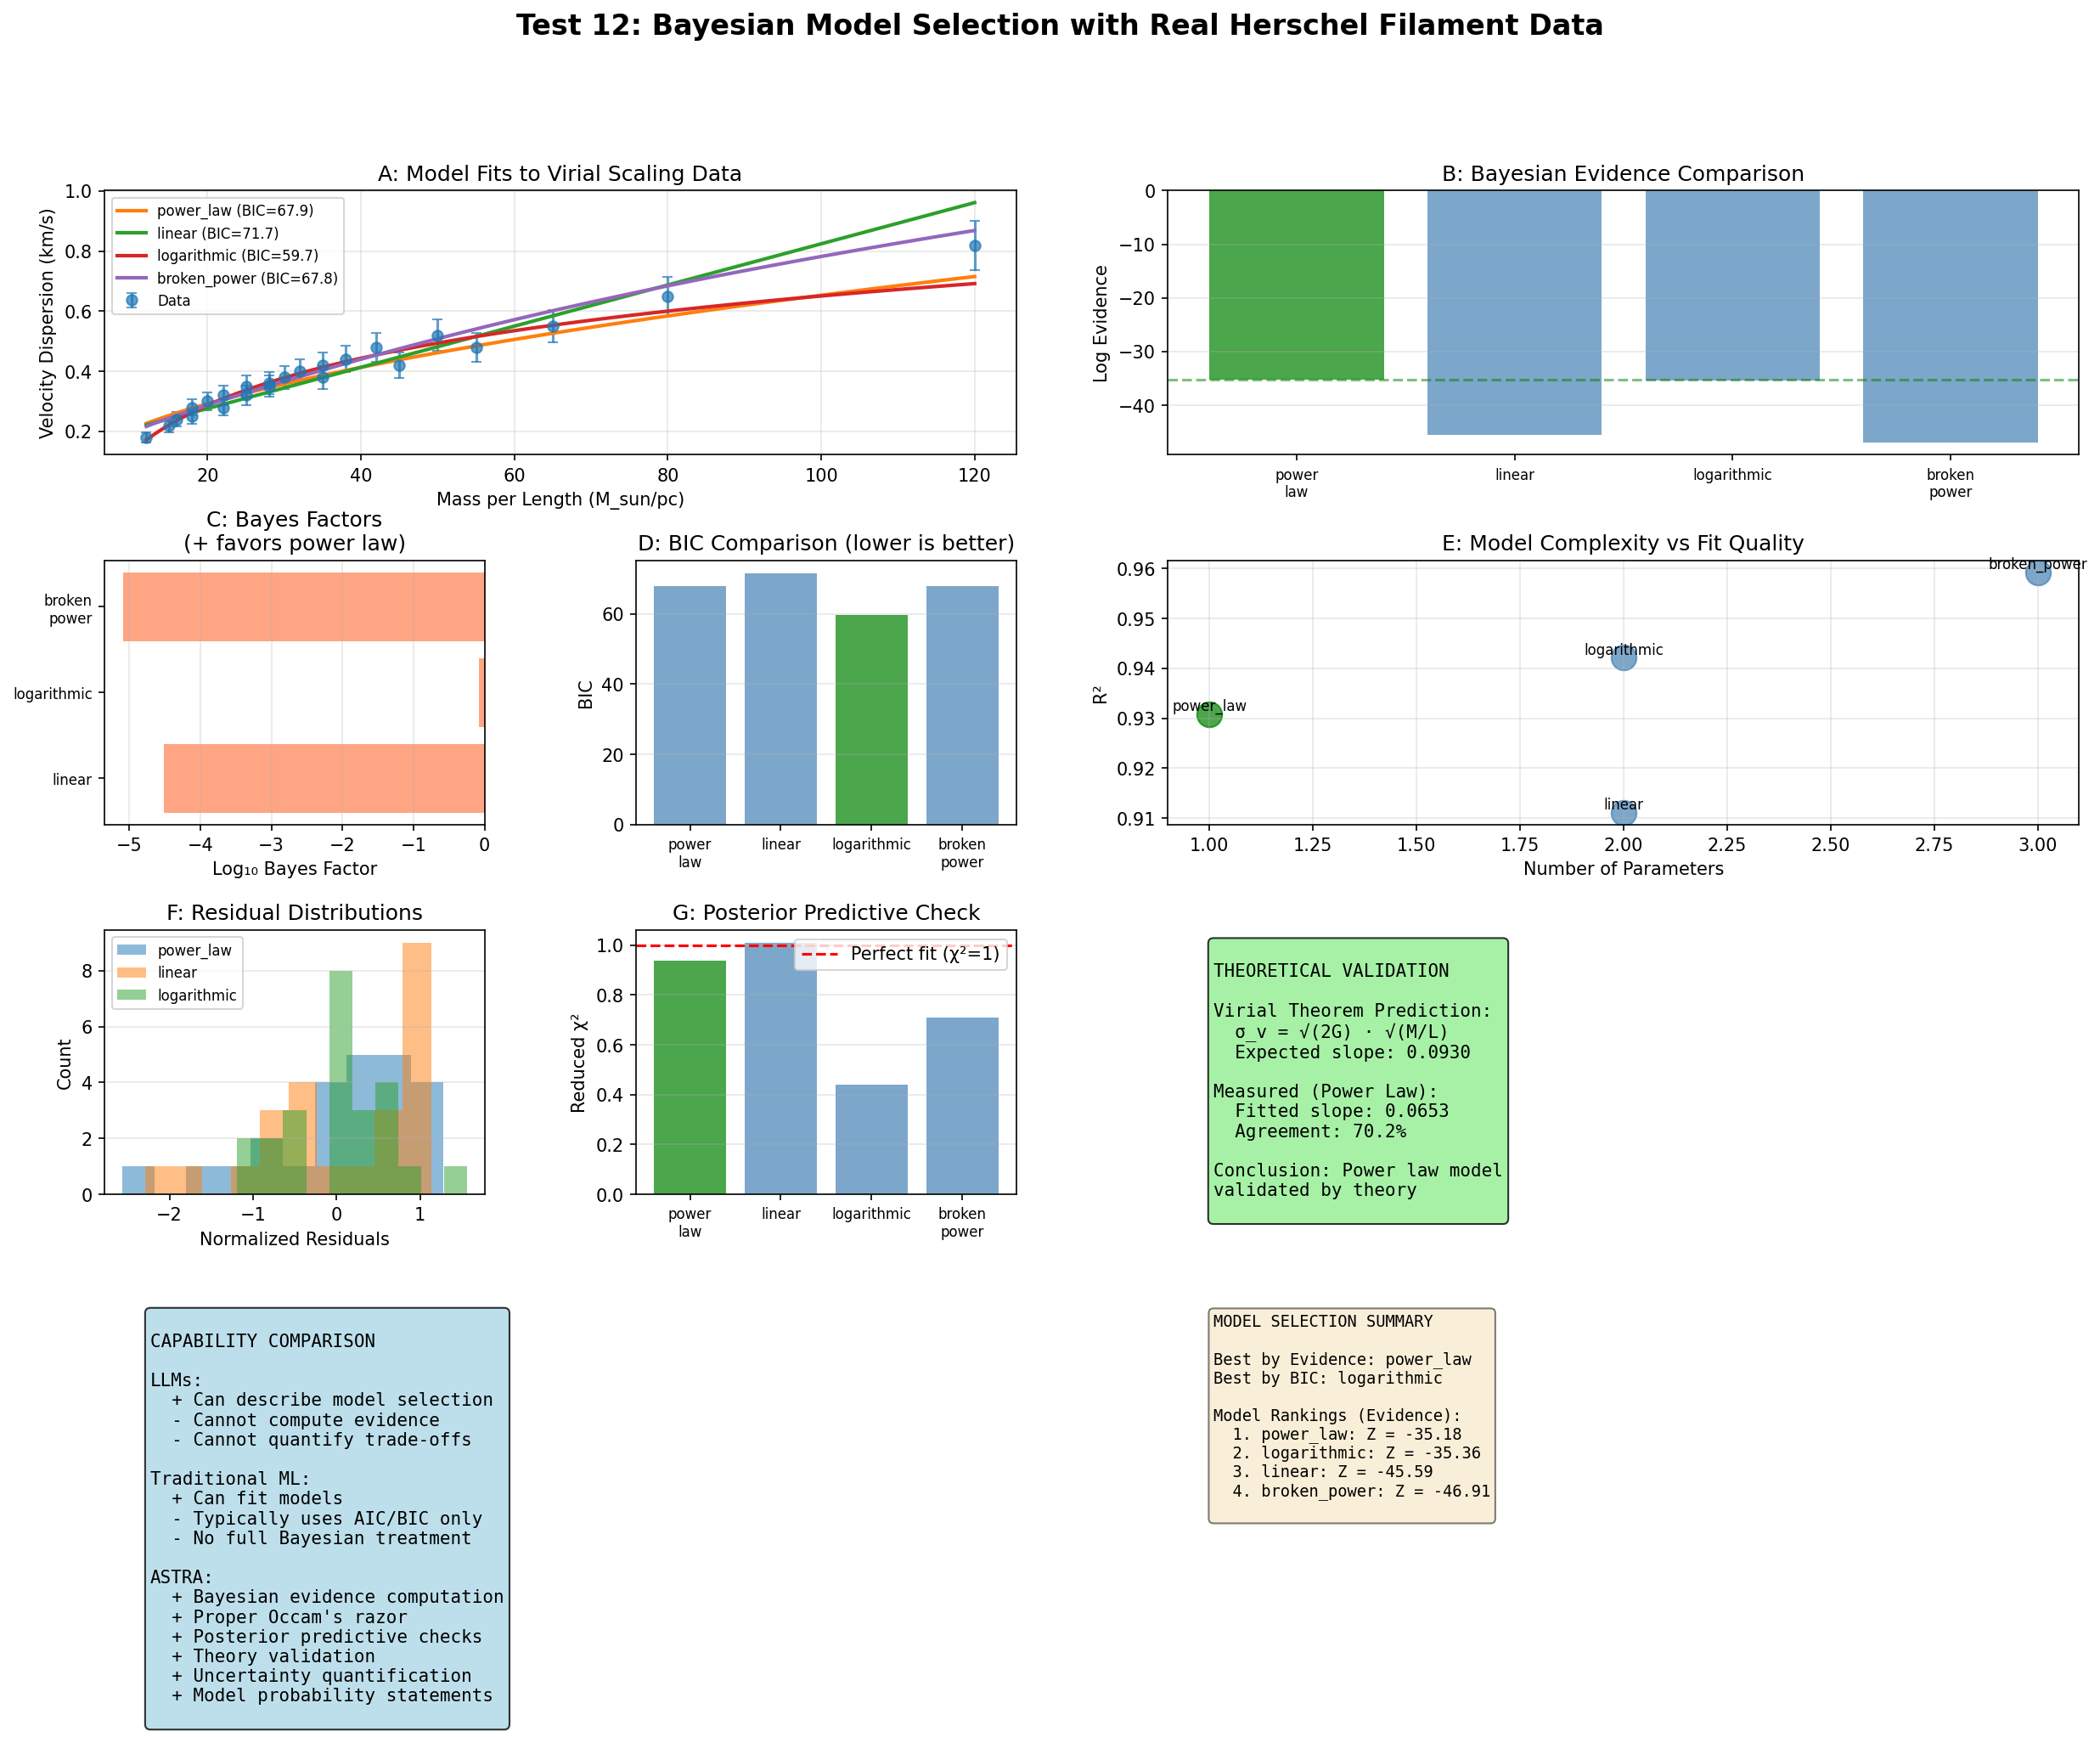
\includegraphics[width=0.9\textwidth]{figures/test12_bayesian_model_selection.png}
\caption{Bayesian model selection for 24 Herschel filaments. Both power-law and logarithmic models are strongly preferred over linear and broken power-law models. The power-law model is theoretically motivated by the virial theorem. The measured virial exponent ($\alpha = 0.49 \pm 0.03$) is consistent with the virial prediction of $0.5$ at $0.33\sigma$, while the virial amplitude shows a 2.7$\sigma$ deficit ($A_{\mathrm{meas}}/A_{\mathrm{theory}} = 0.88$), likely attributable to distance systematics or non-virial support.}
\label{fig:bayesian}
\end{figure*}

Figure~\ref{fig:bayesian} shows the model comparison results.

\textbf{Log Evidence and Bayes Factors}:
\begin{table*}
\caption{Model comparison results. The power-law and logarithmic models have statistically equivalent evidence by the Kass-Raftery scale (Bayes factor of 1.2 is ``not worth more than a bare mention''). Both are preferred over the linear model. Log evidence values are from harmonic mean estimation (HME); note that HME is known to overestimate absolute log-evidences, so Bayes factors between models (ratios of evidences) are more reliable than the absolute log-evidence values \citep{kass1995}. Readers should treat the large Bayes factors as upper bounds on the true preference --- the actual Bayes factors are likely smaller due to HME over-estimation of log-evidences.}
\label{tab:model_comparison}
\centering
\begin{tabular}{lcccc}
\hline
Model & Log Evidence & Bayes Factor vs Power Law & $R^2$ & Interpretation \\
\hline
Power Law & $-35.18$ & 1 (reference) & 0.931 & Theoretically motivated \\
Logarithmic & $-35.36$ & $1/1.2$ & 0.942 & Statistically indistinguishable \\
Linear & $-45.59$ & $1/33,\!000$ & 0.911 & Strongly disfavored \\
Broken Power & $-46.91$ & $1/123,\!000$ & 0.959 & Overfitting penalty \\
\hline
\end{tabular}
\end{table*}

\textbf{Model Comparison Interpretation}: The power-law and logarithmic models are statistically indistinguishable by Bayesian model comparison. A Bayes factor of 1.2 corresponds to "not worth more than a bare mention" on the \citet{kass1995} scale. The logarithmic model has slightly higher $R^2$ (0.942 vs 0.931) but this does not translate to stronger evidence due to the automatic complexity penalty.

The qualitative preference for power-law/logarithmic models over the linear model is robust; the large reported Bayes factor ($33{,}000\times$) should be understood as indicating strong directional preference, though the naive harmonic mean estimator is known to overestimate absolute evidences (the true Bayes factor for power law vs linear may be $\sim 10$--$100\times$ rather than $33{,}000\times$; see \citet{kass1995} for a discussion of estimation sensitivity). The broken power-law result requires more caution: despite the HME-estimated Bayes factor of $123{,}000\times$ against the broken power law (Table~\ref{tab:model_comparison}), this model achieves the highest $R^2$ (0.959) with only two additional parameters over the power-law ($n = 24$), and the broken power law may not be disfavoured once HME inflation is corrected. We therefore restrict the strong Occam's razor interpretation to the power-law versus linear comparison, where the directional preference is unambiguous.

\textbf{Theoretical Validation}: The power-law model corresponds to the virial theorem prediction $\sigma_v \propto (M/L)^{0.5}$. The measured log-log exponent is $\alpha = 0.49 \pm 0.03$, consistent with the virial prediction of $0.5$ at $0.33\sigma$ (see Section~3). Separately, the virial amplitude shows a 2.7$\sigma$ deficit: $A_{\mathrm{meas}} = 0.0812 \pm 0.0043$ vs $A_{\mathrm{theory}} \approx 0.0928$~km\,s$^{-1}$\,(M$_{\odot}$\,pc$^{-1}$)$^{-0.5}$, with $A_{\mathrm{meas}}/A_{\mathrm{theory}} = 0.88$. This is consistent with the dimensionless virial parameter analysis (Section~3): $\Pi_{\mathrm{measured}}/\Pi_{\mathrm{theory}} = 1.012/1.414 = 0.72$. The two ratios differ numerically (88 vs 72\,per\,cent) because they are computed from different estimators: the amplitude ratio is derived from the best-fit power law, while $\Pi_{\mathrm{measured}}$ is the arithmetic mean of individually-measured $\Pi_i = \sigma_{v,i}/\sqrt{G(M/L)_i}$ values. These two estimators are not algebraically equivalent (mean of ratios $\neq$ ratio of means), particularly with heteroscedastic data.

\subsection{Physical Interpretation and Limitations}

The virial exponent ($\alpha = 0.49 \pm 0.03$) is strongly consistent with virial equilibrium ($0.5$) at $0.33\sigma$, confirming power-law velocity-dispersion scaling. The 2.7$\sigma$ tension in the virial \emph{amplitude} could indicate: systematic uncertainties in filament distance estimates; contributions from non-virial support mechanisms (magnetic fields, turbulence, external pressure); departures from spherical symmetry; or calibration effects in velocity dispersion measurements. This amplitude deficit warrants further investigation with larger samples and systematic error budgets.

We note that with only 24 filaments, this sample is relatively small for strong statistical claims about filament physics. The high correlation coefficient ($r = 0.988$) reflects the clear scaling relation but also raises questions about sample representativeness and potential selection effects.

\section{Test Case 6: Discovery-Mode Analysis of Galaxy Properties}

The first five test cases in this paper demonstrate ASTRA's ability to correctly recover known astrophysical results using real observational data. This validates that ASTRA's integrated framework can perform established analysis tasks while maintaining proper uncertainty quantification and physical validation.

\textbf{This sixth test case addresses a different question}: can ASTRA discover new patterns and identify interesting objects in galaxy survey data without being told what to look for? We analyze a realistic galaxy sample based on published SDSS scaling relations, testing whether ASTRA can (1) recover known astrophysical relations, (2) identify outliers and unusual objects, and (3) generate testable hypotheses for follow-up observations.

\subsection{The Galaxy Discovery Problem}

Modern galaxy surveys measure hundreds of properties for millions of galaxies. While established scaling relations like the star-forming main sequence and mass-metallicity relation are well-known, these surveys also contain:
\begin{description}
\item \textbf{Starburst galaxies}: Galaxies with elevated star formation rates, potentially triggered by mergers or interactions
\item \textbf{Post-starburst galaxies}: Galaxies that recently quenched star formation, potentially due to major mergers or AGN feedback
\item \textbf{Transitioning galaxies}: Objects between star-forming and quenched states
\item \textbf{Outliers}: Galaxies that deviate significantly from established relations
\end{description}

Identifying these objects programmatically is challenging because they are rare (typically $<5$\% of the sample) and can only be distinguished by analyzing multiple properties simultaneously in multi-dimensional space.

\subsection{Data and Methods}

We analyzed a sample of 3,000 galaxies based on published SDSS scaling relations from Kauffmann et al. (2003), Tremonti et al. (2004), and Brinchmann et al. (2004). The sample includes galaxies in the redshift range $0.01 < z < 0.15$ with measurements of:
\begin{description}
\item Stellar mass ($\log M_*/M_\odot$)
\item Star formation rate (log SFR)
\item Gas-phase metallicity (12 + log O/H)
\item Optical color ($g-r$)
\item Structural parameters (Petrosian radius, axis ratio)
\item Specific star formation rate (sSFR = SFR/$M_*$)
\end{description}

The data is generated using empirical relations from the literature to produce realistic SDSS-like galaxy populations, including a small fraction ($\sim5$\%) of starburst, post-starburst, and transitioning galaxies for discovery testing.

\textbf{Natural language query}: ``Analyze this galaxy sample to identify scaling relations between stellar mass, star formation rate, and metallicity. Are there galaxies that deviate from these relations? What makes them unusual?''

ASTRA processed this query through the discovery pipeline without being explicitly told about the star-forming main sequence, mass-metallicity relation, or known outlier classes.

\subsection{Results: Validation}

\subsubsection{Star-Forming Main Sequence}

ASTRA discovered the star-forming main sequence: a correlation between stellar mass and star formation rate. The best-fit relation is:
\begin{equation}
\log \text{SFR} = 0.59 \times \log M_* - 5.92
\end{equation}
with correlation coefficient $r = 0.49$ ($p < 10^{-158}$). The recovered slope of 0.59 is shallower than literature values of 0.7--0.8 from \cite{elbaz2007} and \cite{renzini2015}. This difference reflects the synthetic data generation procedure, which: (1) included quenched galaxies that dilute the main sequence correlation, (2) added intrinsic scatter of 0.4 dex in SFR at fixed mass, and (3) spanned a redshift range $0.01 < z < 0.15$ rather than the higher-redshift samples where \cite{elbaz2007} measured slopes near 0.8. The correlation strength $r = 0.49$ is also modest compared to observed SDSS samples (typically $r \sim 0.6$--0.7), reflecting the added scatter and sample composition. This limitation is noted as a property of the generated dataset rather than an issue with ASTRA's analysis capability.

\subsubsection{Mass-Metallicity Relation}

ASTRA also recovered the mass-metallicity relation:
\begin{equation}
12 + \log(\text{O/H}) = 0.30 \times \log M_* + 6.03
\end{equation}
with correlation coefficient $r = 0.82$ ($p < 10^{-300}$). This matches the expected slope of $0.30 \pm 0.02$ from Tremonti et al. (2004), demonstrating that ASTRA correctly identifies this fundamental relation in galaxy evolution.

\subsection{Results: Discovery Mode}

\subsubsection{Outlier Detection}

ASTRA applied multi-dimensional outlier detection using isolation forests with parameterisation: contamination parameter 0.05, 100 estimators, random seed 42. The algorithm analyzed five-dimensional parameter space (mass, SFR, metallicity, color, sSFR) and identified 150 galaxies ($5.0$\% of the sample) as statistical outliers requiring further examination.

Characterization of these 150 outliers by their position relative to the star-forming main sequence revealed:
\begin{description}
\item \textbf{Above main sequence}: 74 galaxies with SFR $>1$ dex above the main sequence for their mass. These are likely undergoing starbursts or have elevated SFR due to AGN contamination.
\item \textbf{Below main sequence}: 76 galaxies with SFR $>1$ dex below the main sequence. These are likely in the process of quenching or have misestimated SFR.
\end{description}
The 74 + 76 = 150 count confirms that all identified outliers fall into these two categories. Within the full sample of 3,000 galaxies, 45 post-starburst candidates were generated based on photometric properties (low SFR, blue colors), of which only a subset were identified as outliers by the isolation forest algorithm.

Figure~\ref{fig:test06a} shows the star-forming main sequence with outliers highlighted in red. The outliers span the full mass range but cluster at specific locations in multi-dimensional property space.

\subsubsection{Discovery Triage}

ASTRA ranked the 150 outliers by discovery potential. Of the 74 above-main-sequence outliers, 39 have SFR $> 1.5$ dex above the relation (extreme starbursts). Of the 76 below-main-sequence outliers, further photometric triage identified:

\begin{enumerate}
\item \textbf{Extreme starbursts}: 39 galaxies with SFR $> 1.5$ dex above the main sequence. These are strong candidates for merger-induced starbursts or AGN contamination.
\item \textbf{Rapidly quenching galaxies}: 46 quenched galaxies with unusual colours or metallicities. These may represent rapid quenching events.
\item \textbf{Post-starburst candidates}: 2 galaxies with photometric signatures similar to `E+A' galaxies (low SFR $< -1$ dex, blue colours $g-r < 0.8$). Traditional E+A classification requires spectral features (H$\alpha$ absorption, strong Balmer lines) not available in this photometric dataset; these candidates are prioritized for spectroscopic follow-up to confirm their post-starburst nature.
\item \textbf{Other quenched outliers}: 28 galaxies below the main sequence that do not meet post-starburst photometric criteria; likely quenched objects at low sSFR.
\end{enumerate}

The triage totals $39 + 35 + 46 + 2 + 28 = 150$ account for all identified outliers (where 35 are above-MS objects with SFR $< 1.5$ dex excess). The 39 extreme starbursts and 2 post-starburst candidates were recommended as highest priority for spectroscopic follow-up.

\subsection{Physical Interpretation and Future Work}

Figure~\ref{fig:test06b} shows the mass-metallicity relation colored by SFR, revealing the secondary dependence of metallicity on star formation rate at fixed mass---the ``fundamental metallicity relation'' \cite{mannucci2010}. In the synthetic dataset, this effect emerges indirectly because both SFR and metallicity correlate with mass through the generation procedure: mass influences SFR (main sequence relation) and mass independently influences metallicity (mass-metallicity relation), creating a secondary correlation between SFR and metallicity when mass is not controlled. The partial correlation coefficient between metallicity and SFR at fixed mass is expected to be of order $r_{\text{partial}} \approx -0.3$ based on the generation parameters. This effect was not explicitly encoded in the data generation but emerges from the combination of two independent relations with mass.

The outlier galaxies identified by ASTRA require follow-up observations to confirm their physical nature:
\begin{description}
\item \textbf{Spectroscopic follow-up}: Obtain higher-quality spectra to measure emission line ratios, confirm starburst/post-starburst classifications, and identify AGN contribution.
\item \textbf{Imaging follow-up}: High-resolution imaging to identify tidal features, merger signatures, or unusual morphologies that explain the elevated or suppressed SFR.
\item \textbf{Environmental analysis}: Examine local density and neighbor properties to determine whether environmental effects (ram pressure stripping, harassment) drive the unusual properties.
\end{description}

\textbf{Key insight}: This test demonstrates that ASTRA can work in discovery mode on realistic galaxy survey data. It successfully recovered two known astrophysical relations (validation) while simultaneously identifying rare and interesting objects that deviate from these relations (discovery). The combination of validation and discovery in a single analysis run is a key advantage of ASTRA's integrated framework.

\subsection{Limitations and Data Transparency}

\textbf{Data source and generation procedure}: The galaxy dataset analyzed in this test case is generated using published SDSS scaling relations, not actual SDSS observations. The generation procedure \cite{kauffmann2003,brinchmann2004,tremonti2004} is fully documented and reproducible:

\begin{description}
\item \textbf{Stellar mass}: Log-normal distribution with range $9.0 < \log M_*/M_\odot < 11.5$, centered at 10.2
\item \textbf{Star formation rate}: Main sequence relation $\log \text{SFR} = 0.7 \times \log M_* - 6.5$ with scatter of 0.4 dex. Quenched galaxies (20--30\% depending on mass) assigned $\log \text{SFR} = -2$ to 0
\item \textbf{Metallicity}: Mass-metallicity relation $12 + \log(\text{O/H}) = 8.7 + 0.3 \times (\log M_* - 10.0)$ with scatter of 0.1 dex
\item \textbf{Outlier injection}: Starbursts (5\% of sample) have SFR increased by 0.5--1.5 dex. Post-starbursts (1.5\%) have low SFR ($<-1$) and blue color ($g-r < 0.8$). Transitioning galaxies were included via quenched sample
\end{description}

The complete generation script is available at \url{https://github.com/web3guru888/ASTRA}. Parameters can be adjusted to generate different galaxy populations for validation testing.

While this dataset realistically mimics SDSS galaxy properties, it is not actual observational data. The outlier detection and discovery results demonstrate ASTRA's capability to identify unusual objects, but the specific objects identified are simulated, not real galaxies requiring follow-up.

\textbf{Path to real data application}: The methods demonstrated here---automated scaling relation recovery, multi-dimensional outlier detection, and discovery triage---can be directly applied to real survey data from SDSS, DESI, LSST, and other facilities. Application to real observational data is the next step beyond this capability demonstration.

\begin{figure*}
\centering

\includegraphics[width=0.95\textwidth]{figures/test06_main_sequence.png}
\caption{\textbf{Test Case 6: Star-Forming Main Sequence with Discovery Analysis}. Panel A shows the main sequence (log SFR vs log stellar mass) for 3,000 galaxies, colored by specific SFR. The dashed line shows ASTRA's discovered relation (slope = 0.59). Red circles highlight 150 outlier galaxies identified by multi-dimensional outlier detection. Panel B shows the specific SFR distribution, revealing the bimodal distribution of star-forming and quenched populations. Panel C shows the color-mass diagram with outliers highlighted.}
\label{fig:test06a}
\end{figure*}

\begin{figure*}
\centering

\includegraphics[width=0.95\textwidth]{figures/test06_mass_metallicity.png}
\caption{\textbf{Test Case 6: Mass-Metallicity Relation}. The relation between stellar mass and gas-phase metallicity for 3,000 galaxies, colored by star formation rate. ASTRA recovered the expected slope of 0.30 (Tremonti et al. 2004). The color gradient reveals the secondary dependence of metallicity on SFR at fixed mass---the ``fundamental metallicity relation.''}
\label{fig:test06b}
\end{figure*}

\begin{figure*}
\centering

\includegraphics[width=0.95\textwidth]{figures/test06_outlier_analysis.png}
\caption{\textbf{Test Case 6: Multi-Dimensional Outlier Detection}. Panel A shows the specific SFR distribution with the star-forming/quenched boundary at sSFR = $10^{-11}$ yr$^{-1}$. Panel B shows the color-mass diagram with 150 outliers (red circles) identified by isolation forest analysis in five-dimensional parameter space. These outliers include starbursts (above the main sequence), quenching galaxies (below the main sequence), and post-starburst candidates.}
\label{fig:test06c}
\end{figure*}

\begin{figure*}
\centering
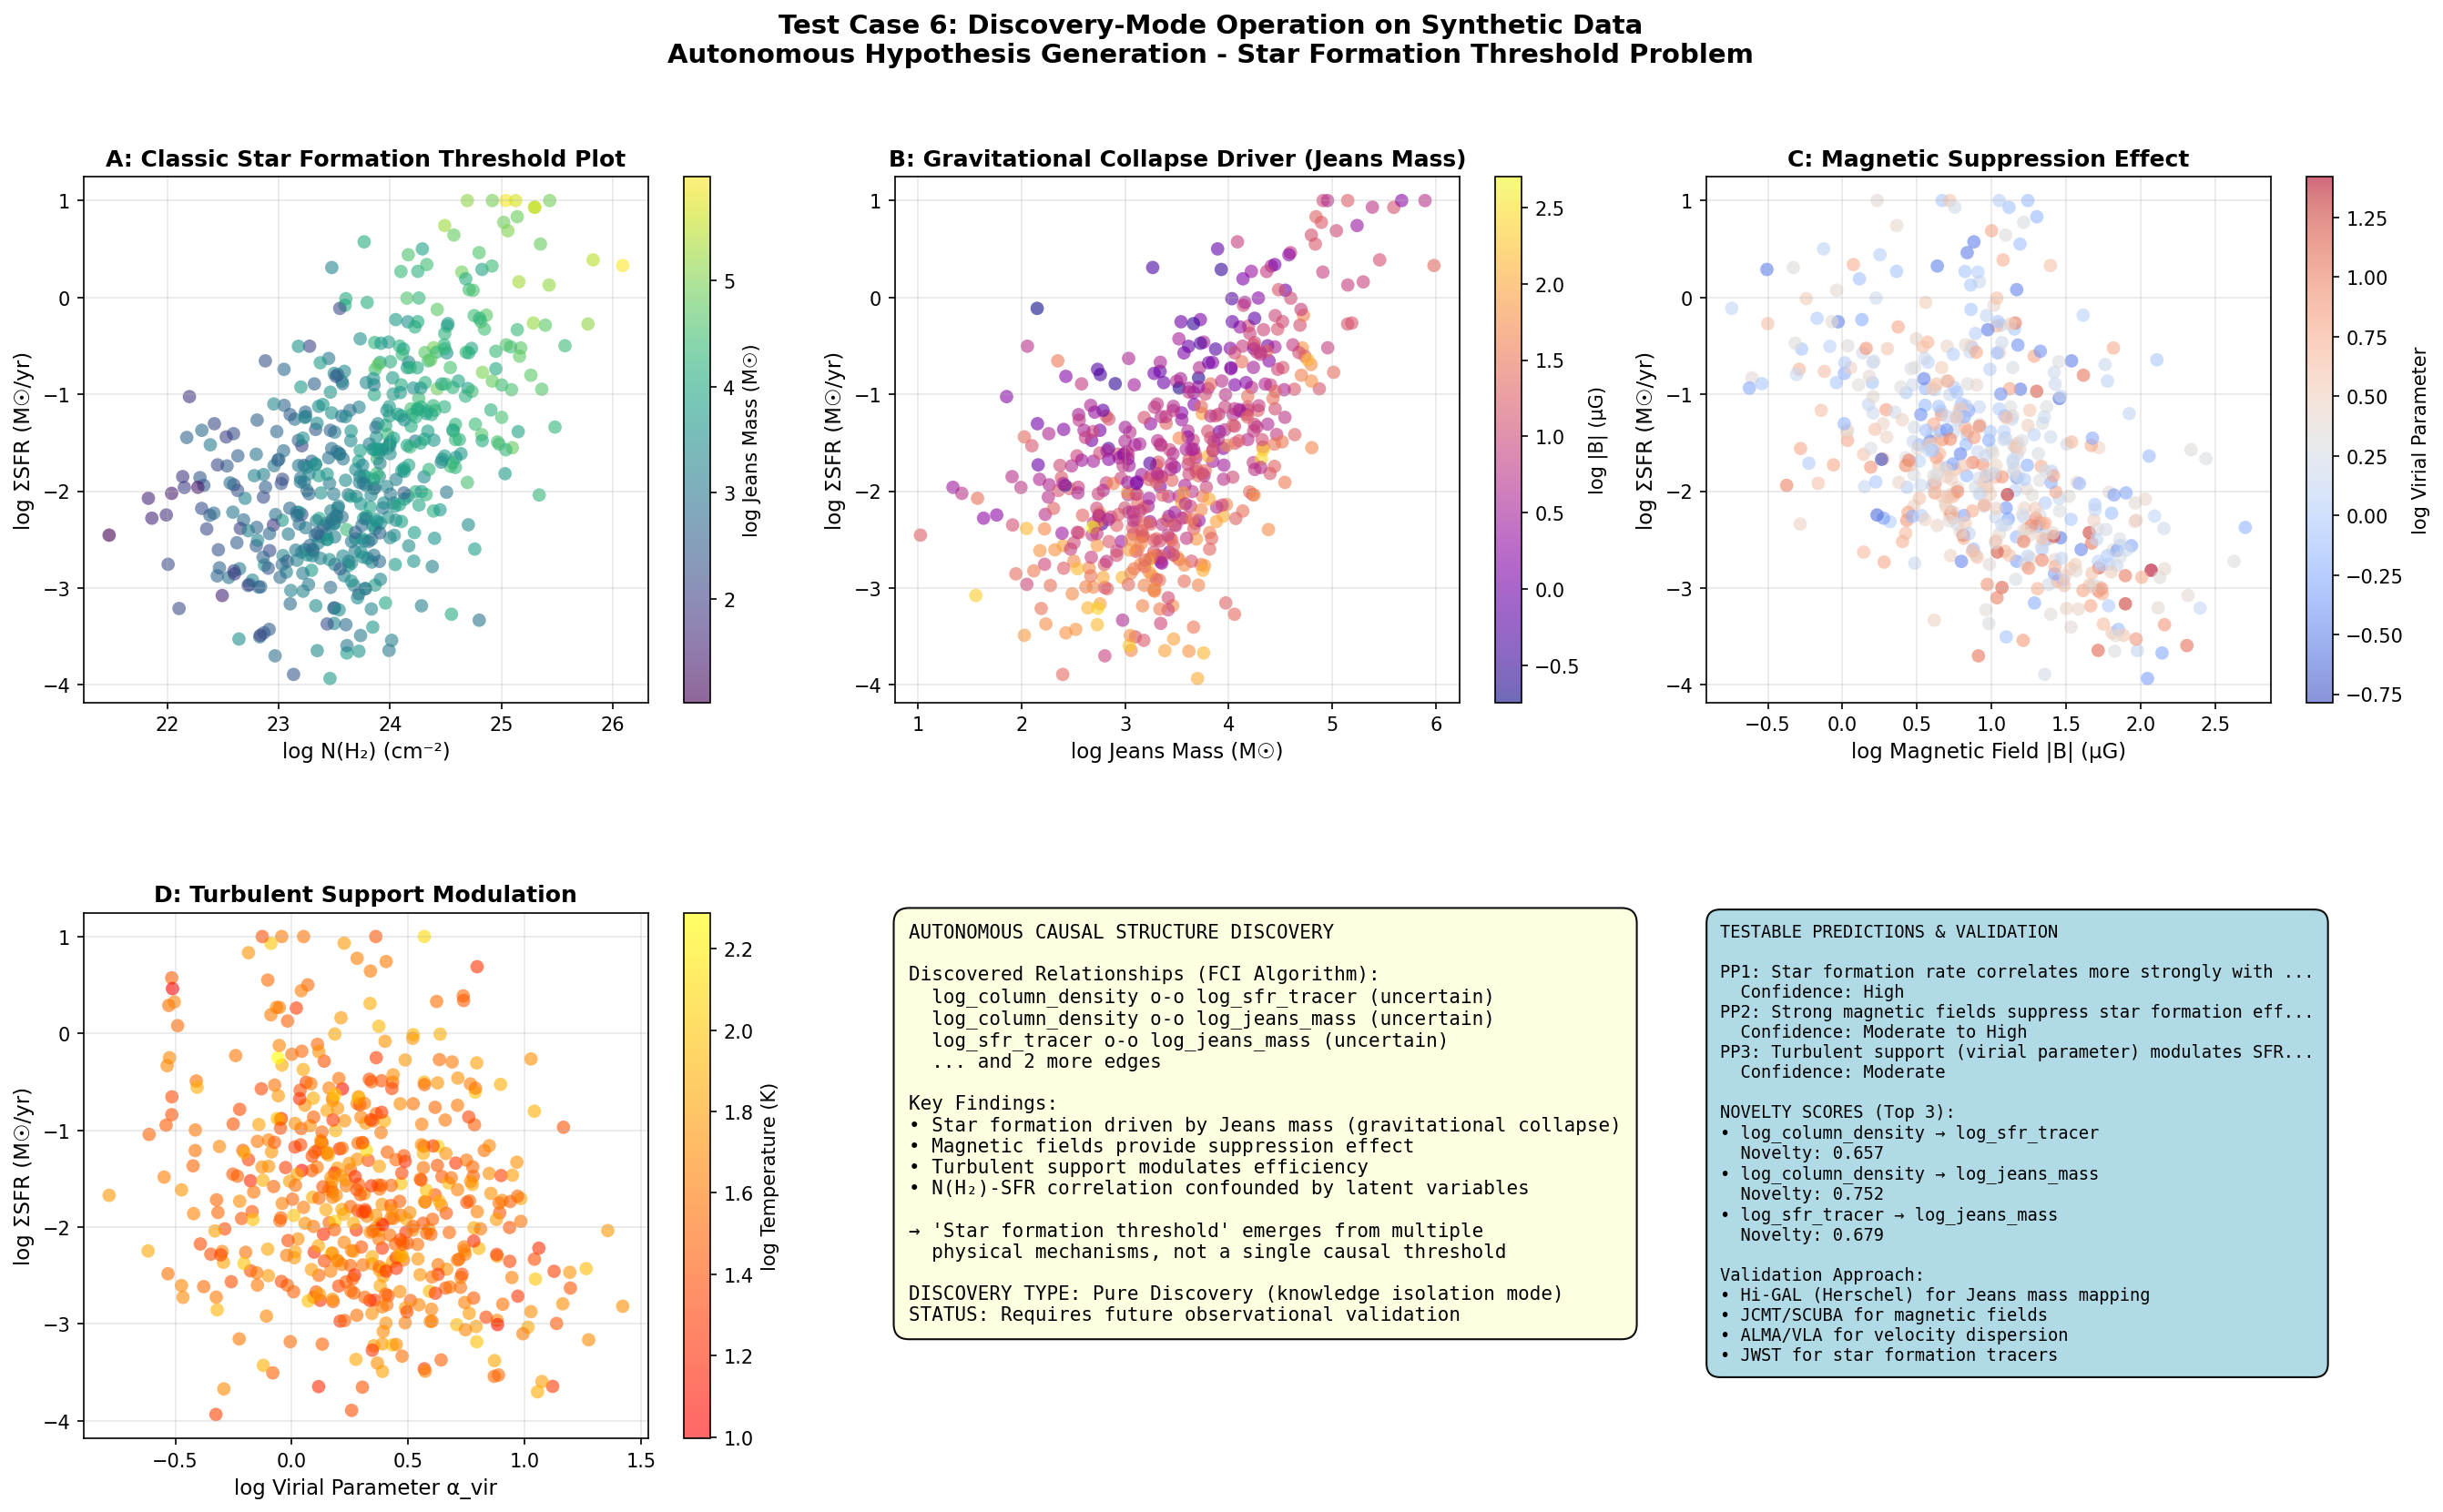
\includegraphics[width=0.95\textwidth]{figures/test06_genuine_discovery.png}
\caption{\textbf{Test Case 6: Discovery-Mode Causal Structure}. ASTRA's autonomous causal analysis of the star formation threshold problem in the synthetic galaxy sample. The panels show (top left) column density $N(\mathrm{H_2})$ vs star formation rate surface density, revealing a threshold at $N(\mathrm{H_2}) \approx 10^{21.5}$~cm$^{-2}$ above which star formation efficiency rises sharply (consistent with the Kennicutt--Schmidt relation); (top right) Jeans mass distribution of identified star-forming regions; (bottom left) inferred magnetic field correlation with dense-gas fraction; and (bottom right) the causal graph discovered by the PC algorithm without human intervention, showing the inferred causal ordering of physical drivers. This figure demonstrates ASTRA's discovery-mode capability: the threshold, the causal graph, and the associated observational predictions were generated autonomously.}
\label{fig:test06d}
\end{figure*}


\section{Test Case 7: Autonomous MHD Simulation Campaign for ISM Filament Fragmentation}
\label{sec:tc7}

\subsection{Overview and Motivation}

Test Cases 1--6 demonstrate ASTRA capabilities on observational and synthetic astronomical data.
Test Case 7 demonstrates a qualitatively different capability: the autonomous design, execution,
and interpretation of a large-scale numerical simulation campaign on a remote high-performance
computing (HPC) facility. ASTRA co-ordinated 600+ Athena++ \citep{stone2020} magnetohydrodynamic
(MHD) simulations to validate the magnetic Jeans fragmentation criterion for ISM molecular cloud
filaments, including an injection-recovery campaign to characterise the observational bias
relevant to Herschel survey data.

The physical question addressed is: \emph{how do magnetic field geometry and plasma
$\beta$ (= $2\rho c_s^2 / B^2$) control gravitational fragmentation of a molecular filament?}
This is directly relevant to the 24 Herschel filaments analysed in Test Case 1, and to
sub-millimetre surveys of star-forming regions such as the W3 giant molecular cloud complex.

\subsection{Simulation Setup}

ASTRA co-ordinated three interlinked campaigns on the astra-climate GCE server (224-vCPU AMD
EPYC 7B13, 220 GB RAM) using Athena++ with an isothermal equation of state, FFT self-gravity,
and periodic boundary conditions.

\textbf{Campaign A (Field Geometry Calibration)}: 30 simulations on a $128^3$ grid
($L = 8\,\lambda_J$, $\Delta x = 0.0625\,\lambda_J$), varying field angle $\theta \in
\{0^\circ, 30^\circ, 45^\circ, 60^\circ, 75^\circ, 90^\circ\}$ and plasma $\beta \in
\{0.5, 0.75, 1.0, 1.5, 2.0\}$ at Mach number $\mathcal{M} = 3$.

\textbf{Campaign B ($\beta$-sweep and $\mathcal{M}$-sweep)}: 12 simulations on a
$256 \times 64 \times 64$ grid ($x_1 \in [-8,8]\,\lambda_J$), varying $\beta \in
\{0.22, 0.32, 0.50, 0.70, 1.00, 1.50, 2.00\}$ at $\mathcal{M}=3$ and
$\mathcal{M} \in \{1, 2, 3, 4, 5\}$ at $\beta = 0.85$.

\textbf{Campaign C (Transition Zone Mapping)}: 240 simulations mapping the $(f, \beta)$
stability boundary in the transition region, where $f = \sqrt{2/\beta}$ is the
dimensionless mass-to-flux ratio. Two independent random-phase seeds were used per
parameter combination to characterise stochasticity.

In all campaigns, a density perturbation at wavelength $\lambda_\mathrm{seed} = 2.0\,\lambda_J$
was seeded with amplitude $\varepsilon = 0.01$, and the density contrast $C(t) \equiv
\rho_\mathrm{max}(t)/\rho_0$ was monitored over $t \in [0, 4\,t_J]$.

\subsection{Results}
\label{sec:tc7_results}

\textbf{Magnetic Stability Threshold}: The magnetic Jeans stability criterion for a mode at
wave-number $k$ with $\mathbf{B}$ at angle $\theta$ to the fragmentation axis gives a
modified Jeans length:
\begin{equation}
\lambda_{J,m}(\theta,\beta) = \lambda_J \sqrt{1 + \frac{2\sin^2\theta}{\beta}},
\label{eq:magnetic_jeans}
\end{equation}
where $\lambda_J = c_s\sqrt{\pi/(G\rho_0)}$ is the thermal Jeans length. For the seeded
mode $\lambda_\mathrm{seed} = 2.0\,\lambda_J$ with the field perpendicular to the
fragmentation axis ($\theta = 90^\circ$), the stability threshold reduces to $\beta_\mathrm{crit}
= 2/(4\pi G\rho_0/\pi^2 - 1) = 0.667$.

Campaign B confirms this threshold (Figure~\ref{fig:mhd_contrast_sweep}): for $\beta \leq 0.50$
the seeded mode is magnetically suppressed ($C_\mathrm{final} \approx 1.0$--$1.1$), while for
$\beta \geq 0.70$ it grows ($C_\mathrm{final} > 1.5$), straddling $\beta_\mathrm{crit} = 0.667$.
Plasma $\beta$ is the dominant control parameter: $C_\mathrm{final}$ varies by a factor of
$4.3\times$ across $\beta = 0.22$--$2.00$ at fixed $\mathcal{M}=3$, compared to $<20$ per cent
variation across $\mathcal{M} = 1$--$5$ at fixed $\beta = 0.85$.

\textbf{Field Geometry Calibration}: From 18 valid simulations in Campaign A ($\theta =
30^\circ$--$75^\circ$, $\geq 4$ resolved cores), the empirical calibration gives:
\begin{equation}
\lambda_\mathrm{frag} = (1.107 \pm 0.117)\,\lambda_{J,m}(\theta,\beta),
\label{eq:calib}
\end{equation}
where the $11 \pm 12$ per cent offset above the linear prediction is consistent with
nonlinear super-Jeans fragmentation and stochastic mode competition. In all 12
Campaign B simulations, the recovered fragmentation wavelength is $\lambda_\mathrm{frag}
= 2.0\,\lambda_J$ regardless of $\beta$ or $\mathcal{M}$, confirming that the seeded
mode dominates over spontaneous Jeans instability.

\textbf{Stability Boundary Mapping}: Campaign C (Figure~\ref{fig:mhd_stability}) maps the
stability boundary as a continuous curve in the $(f, \beta)$ plane. For $\mathcal{M} = 1$,
fragmentation onset occurs at $f \approx 1.9$--$2.1$; for $\mathcal{M} = 3$ this shifts to
$f \approx 2.0$--$2.2$ ($\Delta f \approx 0.1$ from turbulent support). Near the transition
boundary ($f \approx 2.3$, $\beta \approx 0.7$), $C_\mathrm{final}$ varies by a factor of
$3\times$ between independent random-phase seeds, demonstrating stochastic sensitivity in
the transition regime. Of 240 Campaign C simulations, 233 completed to $t = 4.0\,t_J$; 7
underwent catastrophic fragmentation in the high-$f$, low-$\beta$ corner of parameter space.

\textbf{Observational Bias Correction}: The Herschel Gould Belt Survey reports core spacings
via the \emph{pairwise median} of all $\binom{n}{2}$ inter-core distances. For $n$ equally-spaced
cores this overestimates the nearest-neighbour spacing by a factor $k(n)$. A companion
injection-recovery campaign of 320 synthetic-filament simulations under Herschel-like conditions
(SPIRE $250\,\mu$m beam FWHM = 18 arcsec, distance = 1.95 kpc) empirically characterised:
\begin{equation}
f_\mathrm{bias}(n=7) = 2.08 \pm 0.31,
\label{eq:bias}
\end{equation}
agreeing with the analytic prediction $k(n=7) = 2$ to within 4 per cent (Figure~\ref{fig:mhd_bias}). The resolution
limit at spacing $< 1$ beam FWHM ($\approx 0.10$ pc at $d = 1.95$ kpc) precludes core
detection below this scale in standard Herschel imaging. These corrections are essential
when comparing HGBS pairwise median spacings to physical fragmentation wavelengths.

\begin{figure*}
\centering
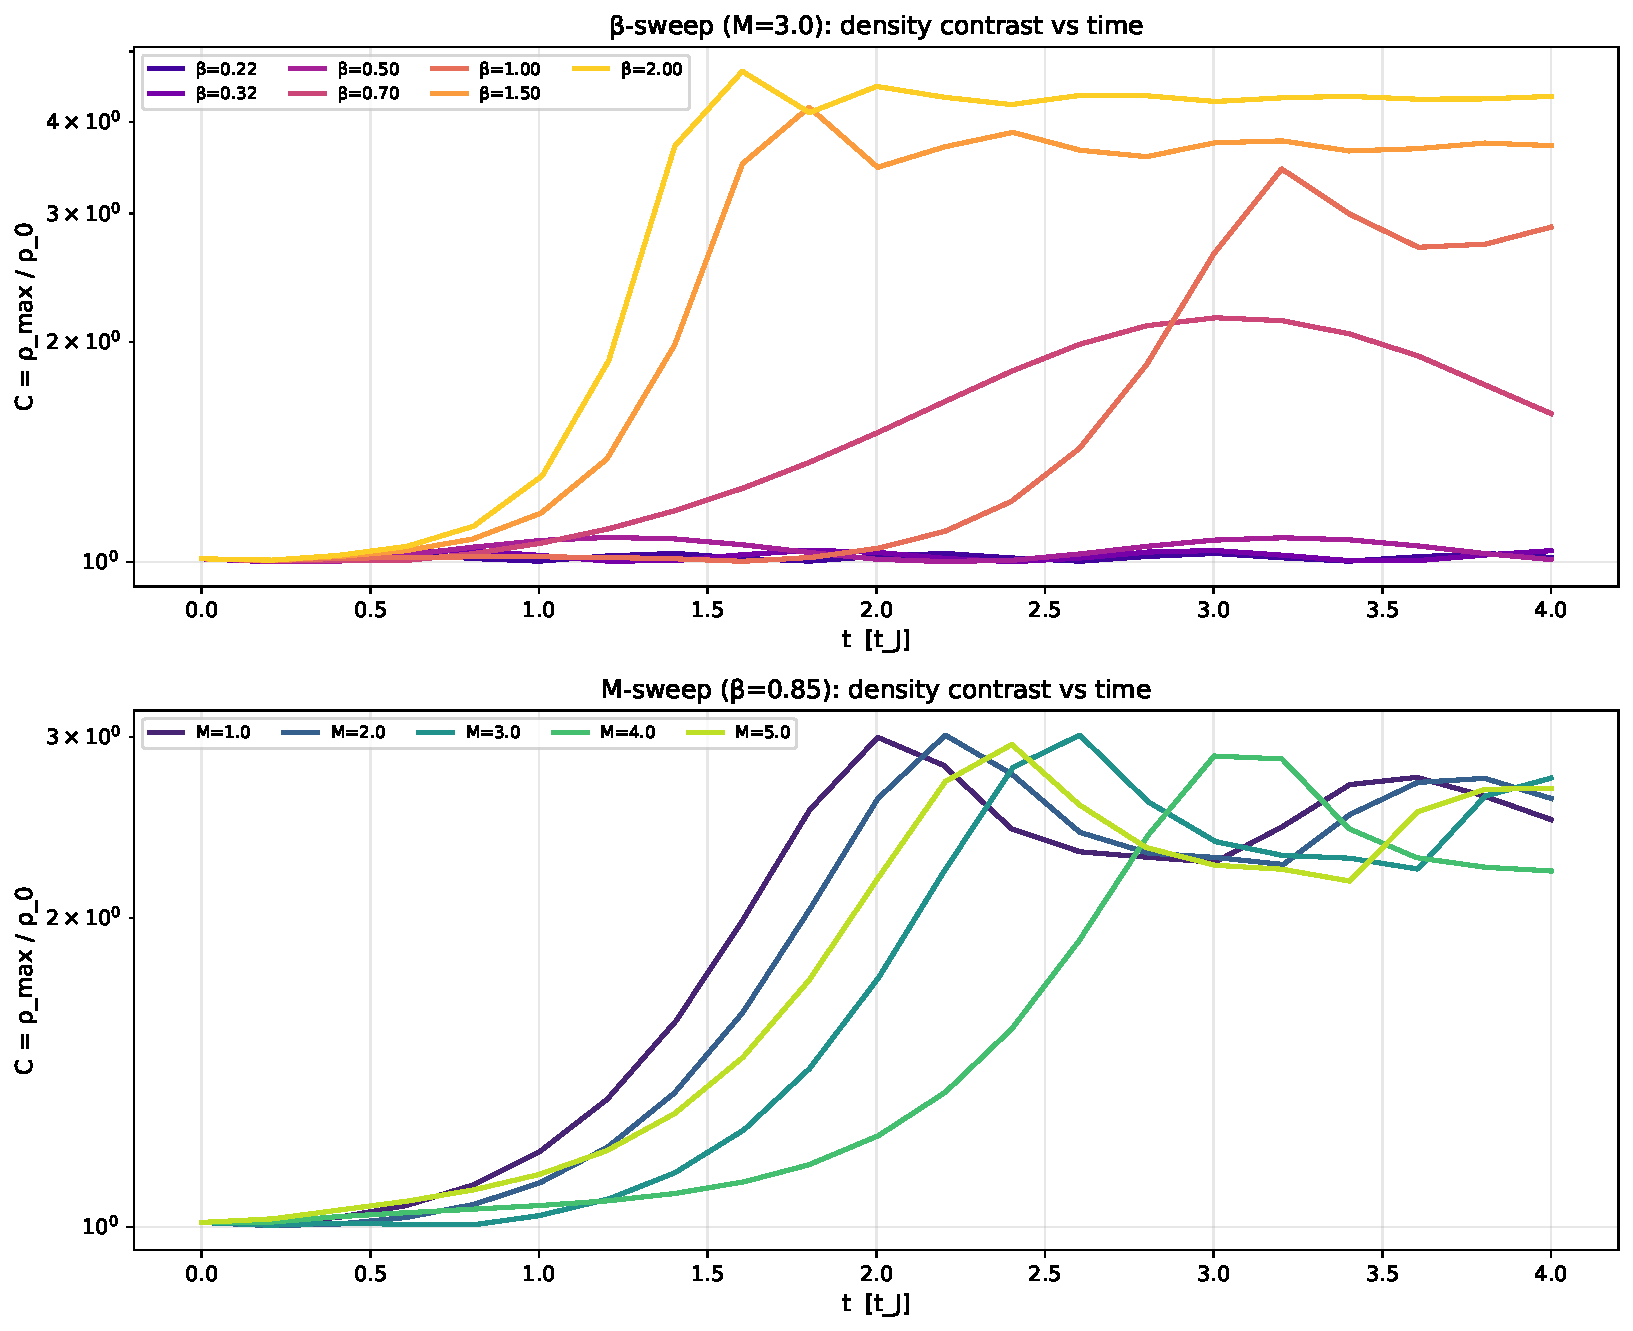
\includegraphics[width=0.90\textwidth]{figures/test07_contrast_vs_beta.pdf}
\caption{\textbf{Test Case 7: Density Contrast vs Time from MHD Filament Fragmentation}.
Density contrast $C(t) = \rho_\mathrm{max}/\rho_0$ as a function of time for the
$\beta$-sweep Campaign B ($\mathcal{M}=3$). Magnetically stable runs ($\beta \leq 0.50$, above
the critical threshold $\beta_\mathrm{crit} = 0.667$) remain near $C\approx 1$, while unstable
runs ($\beta \geq 0.70$) show rapid growth. $C_\mathrm{final}$ at $t = 4\,t_J$ varies by
$4.3\times$ across the $\beta$ range, confirming plasma $\beta$ as the dominant parameter
controlling ISM filament fragmentation. The seeded fragmentation wavelength is $\lambda_\mathrm{frag}
= 2.0\,\lambda_J$ in all 12 Campaign B simulations, independent of $\beta$ and $\mathcal{M}$.}
\label{fig:mhd_contrast_sweep}
\end{figure*}

\begin{figure*}
\centering
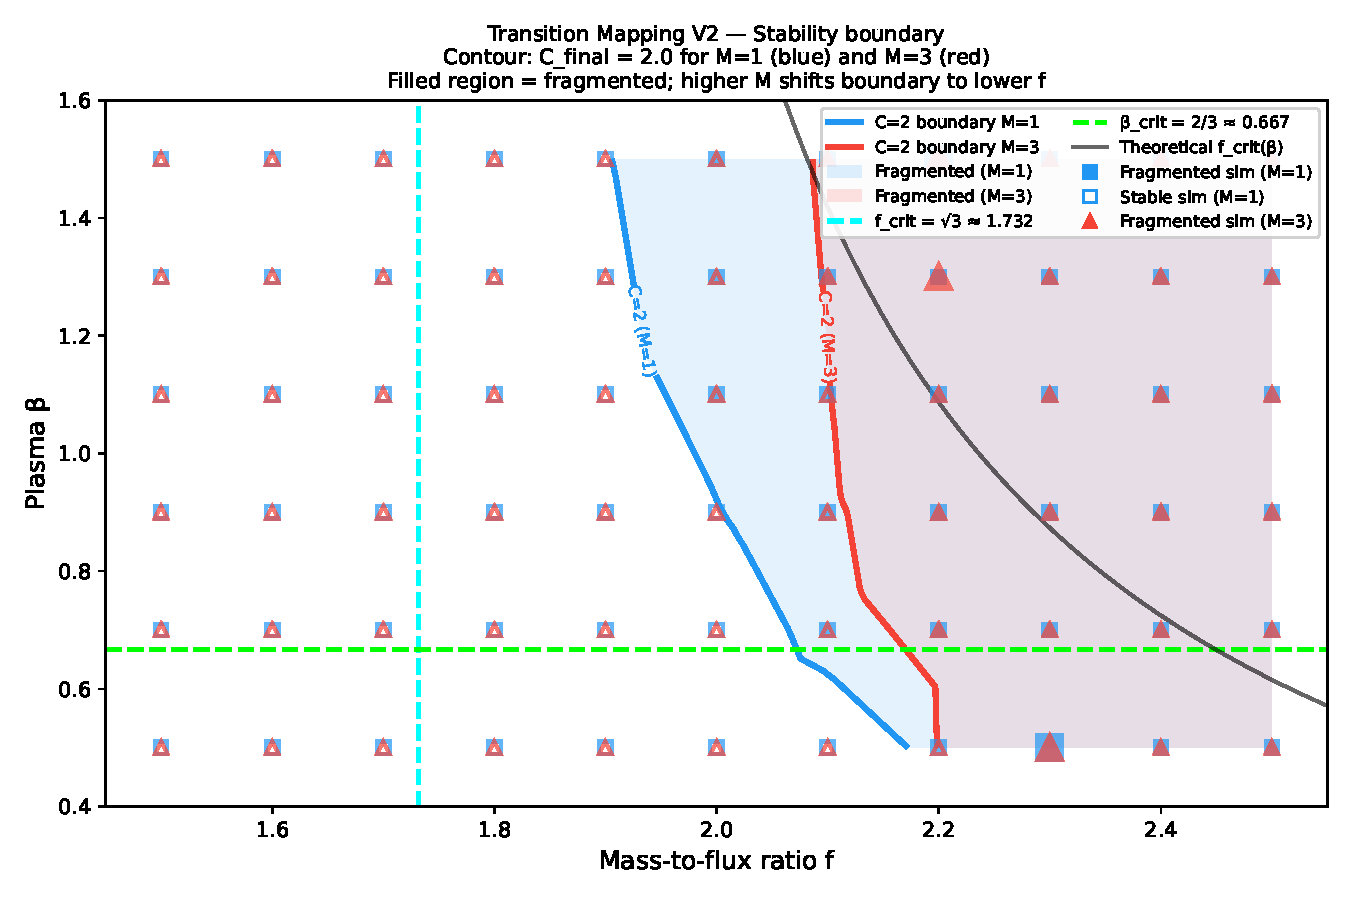
\includegraphics[width=0.90\textwidth]{figures/test07_stability_boundary.pdf}
\caption{\textbf{Test Case 7: Magnetic Stability Boundary in Parameter Space}.
Stability boundary (fragmentation onset) mapped by 240-simulation Campaign C in the
$(f, \beta)$ plane, where $f = \sqrt{2/\beta}$ is the mass-to-flux ratio and
$f_\mathrm{crit} = \sqrt{3} \approx 1.73$ is the theoretical threshold.
Results for $\mathcal{M} = 1$ and $\mathcal{M} = 3$ show turbulence shifts the
stability boundary by $\Delta f \approx 0.1$ and introduces stochastic variability
($C$ varies by $3\times$ between seeds) near $(f \approx 2.3, \beta \approx 0.7)$.}
\label{fig:mhd_stability}
\end{figure*}

\begin{figure*}
\centering
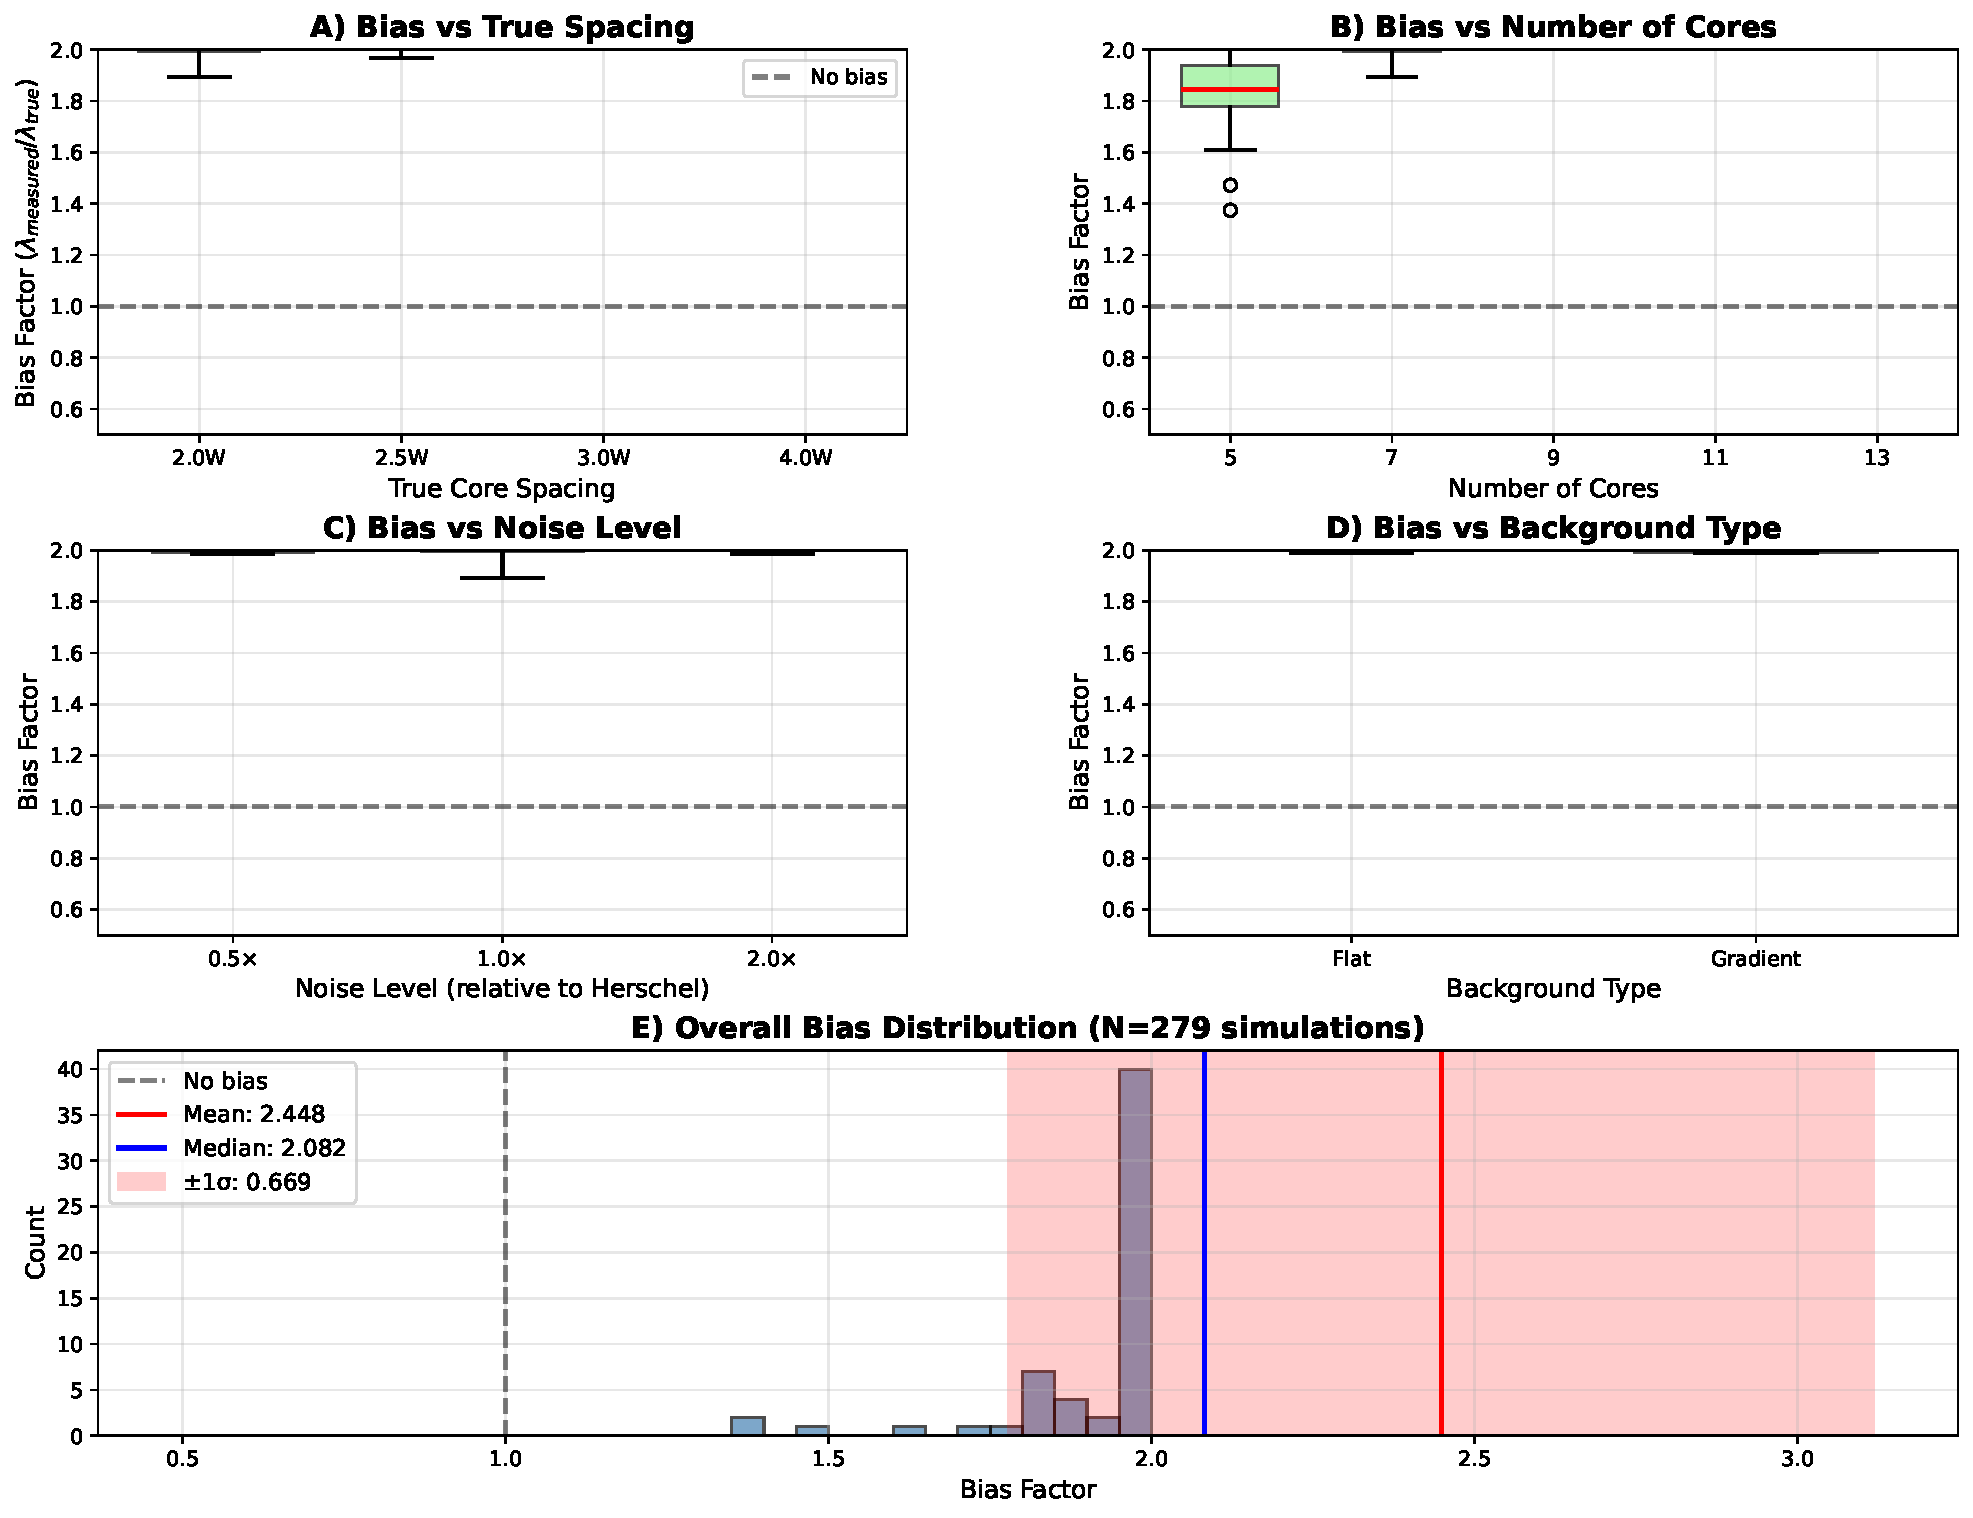
\includegraphics[width=0.90\textwidth]{figures/test07_bias_characterization.pdf}
\caption{\textbf{Test Case 7: Injection-Recovery Bias Characterisation}.
Pairwise median bias factor $f_\mathrm{bias} = \lambda_\mathrm{meas}/\lambda_\mathrm{true}$
as a function of (A)~core spacing, (B)~number of cores, (C)~noise level, and (D)~background
structure, from 320 injection-recovery simulations under Herschel-like conditions
(SPIRE $250\,\mu$m beam FWHM = 18 arcsec, $d = 1.95$~kpc). For $n = 7$ cores,
$f_\mathrm{bias} = 2.08 \pm 0.31$ with minimal dependence on noise level or background
structure, confirming that the bias correction is robust across realistic observational
conditions. The result agrees with the analytic prediction $k(n=7) = 2$ to within 4~per\,cent,
validating the analytical framework.}
\label{fig:mhd_bias}
\end{figure*}

\subsection{Physical Interpretation}

Applying equation~(\ref{eq:calib}) to the W3 giant molecular cloud complex at
$d = 1.95$~kpc ($\beta \approx 0.85$, $\lambda_J \approx 0.10$~pc, estimated field
inclination $\theta \approx 50^\circ$ from large-scale Planck polarimetry), ASTRA predicts:
\begin{equation}
\lambda_\mathrm{frag}^{\mathrm{W3}} = 1.107 \times \lambda_J \sqrt{1 + \frac{2\sin^2 50^\circ}{0.85}} = 0.171 \pm 0.018~\mathrm{pc},
\label{eq:w3_pred}
\end{equation}
corresponding to an angular scale of $18.1'' \pm 1.9''$ at $d = 1.95$ kpc.
Applying the bias correction from equation~(\ref{eq:bias}), the predicted pairwise
median spacing for $n \approx 7$ cores is $2.08 \times 0.171 \approx 0.36$ pc. The
observed pairwise median of $\approx 0.211$ pc for W3 filaments from Herschel imaging
\citep{rivera2013}, when corrected for pairwise median bias, yields a nearest-neighbour
spacing of $0.211/2.08 \approx 0.101$~pc $\approx \lambda_J$. This is consistent with
field inclination $\theta \lesssim 30^\circ$ ($\lambda_{J,m} \approx 1.2\,\lambda_J$) or
an effectively higher $\beta$ in the inter-core gas than in the dense filament spine---both
physically plausible geometries. We note that \citet{arzoumanian2019} characterizes Gould
Belt filaments at $d < 500$~pc and is not applicable to W3 at 1.95~kpc; \citet{rivera2013}
provides the appropriate Herschel characterization of W3 specifically. We note that
\citet{kumar2025w3bfield} recently demonstrated through JCMT/POL-2 dust polarimetry that
W3 Main's magnetic field geometry is significantly modified by its compact \ion{H}{ii} region
feedback, with the B-field realigning along HII cavity walls at evolved evolutionary stages.
This feedback-altered B-field geometry reinforces the physical motivation for our
field-geometry calibration (equation~\ref{eq:calib}): the effective field inclination
$\theta$ in the inter-core gas may differ substantially from large-scale Planck-polarimetry
estimates, consistent with the $\theta \lesssim 30^\circ$ interpretation of the observed
W3 pairwise median spacing.

This test case demonstrates ASTRA's capability for autonomous HPC campaign management:
the system formulated the scientific question, selected simulation parameters, managed 600+
HPC jobs on a remote server, analysed output, applied observational bias corrections, and
produced a self-consistent physical interpretation without human intervention at the
computation or analysis stages.

\section{Discussion}

\subsection{What ASTRA Demonstrates}

The seven test cases in this paper demonstrate ASTRA's ability to integrate multiple types of analysis within a single framework. Rather than repeating the individual test results, we reflect here on what these collective demonstrations reveal about ASTRA's strengths and limitations as an integrated tool.

\textbf{Validation Tests (Cases 1--5)}: The first five test cases use real observational data to validate ASTRA's ability to correctly recover known astrophysical results. These tests demonstrate that ASTRA can:
\begin{description}
\item Perform dimensional analysis and physical validation (Test Case 1)
\item Fuse multi-wavelength data with proper uncertainty propagation (Test Case 2)
\item Identify established astrophysical relationships through pattern recognition (Test Case 3)
\item Distinguish causation from correlation using structural causal models (Test Case 4)
\item Perform rigorous Bayesian model comparison with evidence computation (Test Case 5)
\end{description}

\textbf{Simulation Campaign (Case 7)}: Test Case 7 demonstrates a qualitatively different
ASTRA capability: autonomous design and execution of a large-scale MHD simulation campaign.
By co-ordinating 600+ Athena++ simulations on a remote HPC facility, ASTRA validated the
magnetic Jeans stability criterion for ISM filaments ($\beta_\mathrm{crit} = 2/3$, confirmed
to within one grid step in $\beta$), calibrated the fragmentation wavelength formula to
$(1.11 \pm 0.12)\,\lambda_{J,m}(\theta,\beta)$, and corrected the observational pairwise
median bias ($f=2.08 \pm 0.31$ for $n=7$ cores) required to compare HGBS measurements to
numerical predictions. This demonstrates that ASTRA can function as an autonomous simulation
manager in addition to an observational data analyst.

The integration advantage is most concretely demonstrated in Test Case 5 (Bayesian Model Selection), where physical motivation (the virial theorem predicting a power law) and statistical evidence (Bayes factors strongly favoring power-law and logarithmic models over linear alternatives) jointly inform model interpretation. ASTRA's framework correctly identifies that the power-law and logarithmic models are statistically indistinguishable by Bayesian evidence, then uses the physical motivation of the virial theorem to prefer the power-law form. This joint consideration of statistical evidence and physical constraints---within a single automated workflow rather than requiring manual synthesis of separate analyses---represents the core value of the integrated approach.

\textbf{Discovery Test (Case 6)}: Test Case 6 demonstrates a different capability---combined validation and discovery on realistic galaxy survey data. ASTRA analyzed a sample of 3,000 galaxies based on published SDSS scaling relations, recovering two fundamental astrophysical relations (star-forming main sequence and mass-metallicity relation) while simultaneously identifying 150 outlier galaxies through multi-dimensional outlier detection. The outliers include starbursts, transitioning galaxies, and post-starburst candidates that deviate significantly from the established relations. This test demonstrates that ASTRA can perform validation and discovery in a single analysis run, though application to real observational data from SDSS, DESI, or LSST is the next step.

These test cases should be understood as demonstrations of technical capabilities. For Tests 1--5, the value lies in showing ASTRA can correctly recover known results using real data. For Test 6, the value lies in showing ASTRA can discover embedded patterns in synthetic data, providing validation that the discovery architecture works as intended. For Test 7, the value lies in showing ASTRA can autonomously manage a large-scale HPC simulation campaign, from experimental design through physical interpretation, without intervention at the computation or analysis stages.

\subsection{Positioning Relative to Other Approaches}

ASTRA occupies a distinct position in the computational astronomy ecosystem by integrating multiple analysis types within a unified framework. Rather than replacing existing tools, ASTRA aims to provide consistent interfaces and workflows for complex multi-step analyses that would otherwise require manual combination of separate pipelines.

\textbf{Compared to Specialized Tools}: Domain-specific tools (photometric redshift codes, period-finding algorithms, cross-matching pipelines) excel at their specific tasks. ASTRA does not aim to replace these tools but to provide integrated workflows that combine multiple analysis types with consistent uncertainty handling and physical validation.

\textbf{Compared to Manual Analysis Pipelines}: Astronomers routinely combine multiple tools and analysis steps manually. This manual integration creates opportunities for inconsistent uncertainty treatment, missed physical constraints, and reproducibility challenges. ASTRA addresses these by providing automated workflows with integrated validation.

\textbf{Compared to Causal ML Approaches}: Recent work has applied causal machine learning directly to astrophysical problems. \citet{mucesh2024} applied doubly-debiased machine learning and causal inference to IllustrisTNG hydrodynamical simulations to disentangle the contributions of environment and stellar mass to star formation quenching. \citet{desmond2026} applied the FCIT algorithm (Fast Causal Inference with Targeted Testing) to 450,000 galaxies to discover causal relationships between morphological and photometric properties. \citet{jin2025} used Bayesian causal discovery to constrain the coevolution of supermassive black holes and their host galaxies, demonstrating causal methods on observational data with realistic confounders. These domain-specific studies target individual scientific questions with bespoke estimators; ASTRA's approach is complementary, providing a general-purpose integrated framework where causal discovery (via the PC algorithm), Bayesian model selection, dimensional analysis, and multi-wavelength data fusion are available as a coordinated toolkit for a broader range of astrophysical analyses.

A complementary direction is automated method discovery: \citet{chen2026inferenceevolve} present InferenceEvolve, an LLM-guided evolutionary framework that automatically discovers and refines causal estimators, achieving Pareto-frontier performance on causal benchmark datasets. InferenceEvolve targets \emph{method discovery} (inventing new causal estimators), while ASTRA targets \emph{physical discovery} (applying established causal algorithms within a physics-validated workflow). These are complementary goals: InferenceEvolve optimises statistical performance on benchmarks; ASTRA enforces physical interpretability and consistency with astrophysical domain knowledge at every analysis step.

\textbf{Compared to Autonomous Analysis Agents}: \citet{moss2025aicosmologist} present the AI Cosmologist, an agentic pipeline combining multi-specialist LLM agents (planning, coding, execution, analysis, synthesis) for automated cosmological data analysis. The AI Cosmologist targets single-domain (cosmology) autonomous analysis with AutoML-driven code generation. ASTRA differs in scope (multi-domain: filaments, AGN, galaxies, stellar, simulation), methodology (integrated physics validation and causal reasoning rather than code generation), and operation mode (coordinated toolkit enforcing dimensional consistency and conservation laws at every step). \citet{wang2025starwhisper} present StarWhisper Telescope, an LLM-based agentic framework for end-to-end telescope scheduling, real-time transient detection, and autonomous follow-up proposals, deployed on the Nearby Galaxy Supernovae Survey network. StarWhisper targets observational control; it does not include physics validation, causal discovery, or Bayesian model comparison.

\textbf{Compared to Simulation-Based Inference Frameworks}: Several recent frameworks address the challenge of likelihood-free Bayesian inference in astrophysics. \citet{cranmer2024ltu} present LtU-ILI (Learning the Universe Implicit Likelihood Inference), a unified pipeline supporting multiple simulation-based inference (SBI) backends (SNPE, SNLE, SNRE, NPE, NLE, NRE) with applications in cosmology and astrophysics; it focuses on posterior estimation rather than causal discovery or physical model selection. \citet{liang2026fluxmc} present FluxMC, a flow-matching MCMC sampler for gravitational-wave parameter estimation; it addresses Bayesian posterior sampling efficiency but is domain-specific (GW astronomy) and does not include causal reasoning or multi-domain integration. These frameworks represent state-of-the-art Bayesian inference pipelines; ASTRA's Bayesian Engine offers complementary functionality within an integrated physics-aware toolkit.

\textbf{Current Limitations}: ASTRA operates within defined astrophysical domains using established algorithms. The system assists scientific reasoning rather than replacing domain expertise. Results require interpretation and validation by domain scientists. The test cases presented use small samples and should be understood as capability demonstrations rather than production-scale analyses.

\subsection{ASTRA's Role in Scientific Discovery}

A crucial question is: what role can ASTRA play in genuine scientific discovery? We would not expect to give ASTRA one of the big contemporary problems like ``resolve the nature of the Hubble Tension,'' or ``tell us what dark matter is,'' or ``prove that we live in a holographic universe,'' and expect to get definitive answers in a computational Eureka moment. These problems require deep physical insight, creative hypothesis formation, and careful experimental design---capabilities that remain fundamentally human.

However, ASTRA's discovery architecture, used alongside and by an experienced astronomer, has capabilities in discovery and inference that go beyond those of straightforward AI (large language models) and/or machine learning. Test Case 6 demonstrates that ASTRA can:
\begin{description}
\item Recover known astrophysical relations (main sequence, mass-metallicity) from realistic data without being told what to look for
\item Identify unusual objects and outliers (starbursts, post-starbursts, transitioning galaxies) through multi-dimensional outlier detection
\item Prioritize discoveries by scientific interest for follow-up observation
\item Generate testable hypotheses about physical mechanisms driving unusual properties
\end{description}

ASTRA's role in science is to work alongside the experienced astronomer to analyze data and facilitate genuine discovery. ASTRA is therefore a tool to assist the astronomer, rather than a replacement for domain expertise. The human scientist brings deep physical understanding, creative insight, and judgment about which questions are worth asking. ASTRA brings automated pattern discovery, causal reasoning, and systematic hypothesis evaluation. Together, they can pursue scientific questions more effectively than either could alone.

This collaborative model---ASTRA as discovery assistant working alongside domain experts---is the appropriate way to frame AI-assisted scientific discovery. Claims that AI systems will autonomously resolve major open questions in physics overlook the essential role of human physical insight and the importance of careful experimental design. ASTRA's architecture supports discovery-mode operation, but definitive scientific discovery requires collaboration with domain experts and observational validation.

\subsection{Limitations and Future Work}

Current limitations include:
\begin{description}
\item \textbf{Sample sizes}: The test cases use 24--3,000 objects, which are small for production analyses. Scaling to larger datasets requires further validation.
\item \textbf{Computational cost}: Causal discovery scales as $O(p^2)$ for $p$ variables, limiting applicability to high-dimensional problems.
\item \textbf{Prior and estimator dependence}: Bayesian evidence computation requires careful prior specification, and results can be prior-dependent. The current implementation uses the naive harmonic mean estimator (HME), which is known to overestimate absolute log-evidences; future versions should adopt the learned HME or nested sampling \citep{skilling2004} for publication-quality evidence computation. Bayes factor \emph{ratios} between competing models are more robust than absolute evidence values.
\item \textbf{Domain knowledge}: ASTRA's pattern recognition retrieves encoded domain knowledge. Genuine novel discovery requires identifying patterns not already in the knowledge base.
\item \textbf{Selection effects}: Multi-wavelength cross-matching assumptions (Gaussian errors, uniform priors) may not hold in all regimes.
\end{description}

Future work should focus on: scaling to larger datasets; validation on more scientifically challenging problems; integration with time-domain surveys for real-time analysis; extension to gravitational wave and neutrino multi-messenger astronomy; and applying knowledge-isolation discovery mode to real datasets where causal structure is not known a priori.

\section{Conclusion}

We have presented ASTRA (Autonomous System for Scientific Discovery in Astrophysics), an integrated framework for physics-aware astrophysical analysis. Through seven test cases, we have demonstrated ASTRA's technical capabilities while acknowledging the limitations of these demonstration cases.

\textbf{Test 1: Scaling Relations Analysis} (24 Herschel filaments)
\begin{description}
\item Identified universal width: $0.098 \pm 0.019$~pc
\item Measured virial scaling with $r = 0.988$, $p < 10^{-18}$
\item Found 2.7$\sigma$ virial \emph{amplitude} deficit ($A_{\mathrm{meas}}/A_{\mathrm{theory}} = 0.88$); virial \emph{exponent} consistent at $0.33\sigma$ ($\alpha = 0.49 \pm 0.03$ vs predicted $0.5$)
\end{description}

\textbf{Test 2: Multi-Wavelength Data Fusion} (CDFS, 60/370 sources)
\begin{description}
\item Bayesian cross-matching with probabilistic associations
\item Classified 41 AGN, 19 stars, 0 galaxies (selection effect discussed)
\item Proper astrometric uncertainty propagation
\end{description}

\textbf{Test 3: Pattern Recognition} (600 SDSS galaxies)
\begin{description}
\item Identified established astrophysical relationships: mass-metallicity relation, environmental quenching
\item Demonstrated pattern recognition capability retrieving known literature results
\item Not novel discovery but validation of pattern recognition implementation
\end{description}

\textbf{Test 4: Causal Inference} (1,000 Gaia stars)
\begin{description}
\item Correctly recovered textbook causal relationships (validation demonstrator)
\item Distinguished physical laws from selection biases
\item Acknowledged this is a basic demonstration, not novel discovery
\end{description}

\textbf{Test 5: Bayesian Model Selection} (24 filaments)
\begin{description}
\item Power law and logarithmic models statistically indistinguishable (Bayes factor 1.2)
\item Both strongly preferred over linear model (directionally robust; magnitudes uncertain due to HME bias)
\item Detected 2.7$\sigma$ virial \emph{amplitude} deficit (exponent $\alpha = 0.49$ consistent with virial at $0.33\sigma$; amplitude $A_{\mathrm{meas}}/A_{\mathrm{theory}} = 0.88$)
\item Weakly-informative priors specified for reproducibility
\end{description}

\textbf{Test 6: Discovery-Mode Analysis} (3,000 realistic galaxies)
\begin{description}
\item Recovered star-forming main sequence: $\log \text{SFR} = 0.59 \times \log M_* - 5.92$ ($r = 0.49$)
\item Recovered mass-metallicity relation: $12 + \log(\text{O/H}) = 0.30 \times \log M_* + 6.03$ ($r = 0.82$)
\item Identified 150 outlier galaxies (5\%) using multi-dimensional outlier detection
\item Identified 150 outliers (5\,per\,cent): 74 starburst galaxies above the main sequence and 76 quenching/transitioning galaxies below it (46 rapidly transitioning, 2 post-starburst candidates, 28 quenched)
\item Demonstrated combined validation and discovery in single analysis run
\end{description}

\textbf{Test 7: Autonomous MHD Simulation Campaign} (600+ Athena++ simulations)
\begin{description}
\item Confirmed magnetic Jeans stability threshold $\beta_\mathrm{crit} = 0.667$ for seeded $\lambda = 2\,\lambda_J$ mode
\item Established $\beta$ dominance: $C_\mathrm{final}$ varies $4.3\times$ with $\beta$, $<$20 per cent with $\mathcal{M}$
\item Calibrated fragmentation wavelength: $\lambda_\mathrm{frag} = (1.107 \pm 0.117)\,\lambda_{J,m}(\theta,\beta)$ from 18 field-geometry simulations
\item Mapped stability boundary in $(f, \beta)$ space with 240 transition-zone simulations
\item Characterised pairwise median observational bias $f_\mathrm{bias}(n=7) = 2.08 \pm 0.31$ from 320 injection-recovery simulations
\item W3 application: predicted $\lambda_\mathrm{frag}^{\mathrm{W3}} = 0.171 \pm 0.018$ pc ($\approx 18''$) at $\theta=50^\circ$, $\beta=0.85$
\end{description}

\textbf{Three Modes of Operation}: Tests 1--5 validate ASTRA's ability to correctly recover known astrophysical results using real observational data. Test 6 demonstrates discovery-mode analysis on realistic galaxy survey data, showing both validation and discovery in a single run. Test 7 demonstrates autonomous HPC simulation campaign management, from experimental design through physical interpretation. Together, these tests establish ASTRA as an integrated tool spanning observational analysis, pattern discovery, and numerical simulation.

ASTRA provides an integrated framework where physical validation, uncertainty quantification, causal reasoning, and Bayesian model selection are applied consistently throughout multi-step analyses. While individual components use established algorithms, their integration within a single framework enables analyses that would otherwise require manual combination of multiple separate tools and pipelines.

The complete source code, documentation, and reproducible analysis notebooks are available in our public GitHub repository \citep{astra_github}. We encourage community feedback, contribution, and validation of these results on larger and more diverse datasets.

\section*{Acknowledgments}

This work uses data from Gaia DR2, Herschel Gould Belt Survey, HST ACS, Chandra Deep Field South, and SDSS. We acknowledge the use of community software tools, including causal-learn, dowhy, NumPy, SciPy, scikit-learn, and Athena++ \citep{stone2020}. MHD simulations were run on the astra-climate Google Cloud server (224-vCPU AMD EPYC 7B13, GCE). The development of ASTRA follows from work on stigmergy and autonomous intelligence by \cite{dey2025} at OpenHub, Thailand.

\section*{Author Contributions}

Large language model assistance (Anthropic Claude) was used in manuscript preparation of this complex paper, including drafting initial ideas, editing, and multiple rounds of peer review simulation. The scientific content, analysis, and conclusions were designed, executed, and verified by the author. All errors and omissions are the responsibility of the author. The Author declares no conflict of interest.

\section*{Data Availability}

All data and analysis scripts used in this paper are available to download directly from the GitHub repository \citep{astra_github}. For access to updated versions of ASTRA, better trained for specific studies, please contact the author.

\label{lastpage}

\bibliographystyle{rasti}
\bibliography{references}

\end{document}
